% Options for packages loaded elsewhere
\PassOptionsToPackage{unicode}{hyperref}
\PassOptionsToPackage{hyphens}{url}
%
\documentclass[
]{article}
\usepackage{amsmath,amssymb}
\usepackage{lmodern}
\usepackage{ifxetex,ifluatex}
\ifnum 0\ifxetex 1\fi\ifluatex 1\fi=0 % if pdftex
  \usepackage[T1]{fontenc}
  \usepackage[utf8]{inputenc}
  \usepackage{textcomp} % provide euro and other symbols
\else % if luatex or xetex
  \usepackage{unicode-math}
  \defaultfontfeatures{Scale=MatchLowercase}
  \defaultfontfeatures[\rmfamily]{Ligatures=TeX,Scale=1}
\fi
% Use upquote if available, for straight quotes in verbatim environments
\IfFileExists{upquote.sty}{\usepackage{upquote}}{}
\IfFileExists{microtype.sty}{% use microtype if available
  \usepackage[]{microtype}
  \UseMicrotypeSet[protrusion]{basicmath} % disable protrusion for tt fonts
}{}
\makeatletter
\@ifundefined{KOMAClassName}{% if non-KOMA class
  \IfFileExists{parskip.sty}{%
    \usepackage{parskip}
  }{% else
    \setlength{\parindent}{0pt}
    \setlength{\parskip}{6pt plus 2pt minus 1pt}}
}{% if KOMA class
  \KOMAoptions{parskip=half}}
\makeatother
\usepackage{xcolor}
\IfFileExists{xurl.sty}{\usepackage{xurl}}{} % add URL line breaks if available
\IfFileExists{bookmark.sty}{\usepackage{bookmark}}{\usepackage{hyperref}}
\hypersetup{
  pdftitle={House Pricing},
  hidelinks,
  pdfcreator={LaTeX via pandoc}}
\urlstyle{same} % disable monospaced font for URLs
\usepackage[margin=1in]{geometry}
\usepackage{color}
\usepackage{fancyvrb}
\newcommand{\VerbBar}{|}
\newcommand{\VERB}{\Verb[commandchars=\\\{\}]}
\DefineVerbatimEnvironment{Highlighting}{Verbatim}{commandchars=\\\{\}}
% Add ',fontsize=\small' for more characters per line
\usepackage{framed}
\definecolor{shadecolor}{RGB}{248,248,248}
\newenvironment{Shaded}{\begin{snugshade}}{\end{snugshade}}
\newcommand{\AlertTok}[1]{\textcolor[rgb]{0.94,0.16,0.16}{#1}}
\newcommand{\AnnotationTok}[1]{\textcolor[rgb]{0.56,0.35,0.01}{\textbf{\textit{#1}}}}
\newcommand{\AttributeTok}[1]{\textcolor[rgb]{0.77,0.63,0.00}{#1}}
\newcommand{\BaseNTok}[1]{\textcolor[rgb]{0.00,0.00,0.81}{#1}}
\newcommand{\BuiltInTok}[1]{#1}
\newcommand{\CharTok}[1]{\textcolor[rgb]{0.31,0.60,0.02}{#1}}
\newcommand{\CommentTok}[1]{\textcolor[rgb]{0.56,0.35,0.01}{\textit{#1}}}
\newcommand{\CommentVarTok}[1]{\textcolor[rgb]{0.56,0.35,0.01}{\textbf{\textit{#1}}}}
\newcommand{\ConstantTok}[1]{\textcolor[rgb]{0.00,0.00,0.00}{#1}}
\newcommand{\ControlFlowTok}[1]{\textcolor[rgb]{0.13,0.29,0.53}{\textbf{#1}}}
\newcommand{\DataTypeTok}[1]{\textcolor[rgb]{0.13,0.29,0.53}{#1}}
\newcommand{\DecValTok}[1]{\textcolor[rgb]{0.00,0.00,0.81}{#1}}
\newcommand{\DocumentationTok}[1]{\textcolor[rgb]{0.56,0.35,0.01}{\textbf{\textit{#1}}}}
\newcommand{\ErrorTok}[1]{\textcolor[rgb]{0.64,0.00,0.00}{\textbf{#1}}}
\newcommand{\ExtensionTok}[1]{#1}
\newcommand{\FloatTok}[1]{\textcolor[rgb]{0.00,0.00,0.81}{#1}}
\newcommand{\FunctionTok}[1]{\textcolor[rgb]{0.00,0.00,0.00}{#1}}
\newcommand{\ImportTok}[1]{#1}
\newcommand{\InformationTok}[1]{\textcolor[rgb]{0.56,0.35,0.01}{\textbf{\textit{#1}}}}
\newcommand{\KeywordTok}[1]{\textcolor[rgb]{0.13,0.29,0.53}{\textbf{#1}}}
\newcommand{\NormalTok}[1]{#1}
\newcommand{\OperatorTok}[1]{\textcolor[rgb]{0.81,0.36,0.00}{\textbf{#1}}}
\newcommand{\OtherTok}[1]{\textcolor[rgb]{0.56,0.35,0.01}{#1}}
\newcommand{\PreprocessorTok}[1]{\textcolor[rgb]{0.56,0.35,0.01}{\textit{#1}}}
\newcommand{\RegionMarkerTok}[1]{#1}
\newcommand{\SpecialCharTok}[1]{\textcolor[rgb]{0.00,0.00,0.00}{#1}}
\newcommand{\SpecialStringTok}[1]{\textcolor[rgb]{0.31,0.60,0.02}{#1}}
\newcommand{\StringTok}[1]{\textcolor[rgb]{0.31,0.60,0.02}{#1}}
\newcommand{\VariableTok}[1]{\textcolor[rgb]{0.00,0.00,0.00}{#1}}
\newcommand{\VerbatimStringTok}[1]{\textcolor[rgb]{0.31,0.60,0.02}{#1}}
\newcommand{\WarningTok}[1]{\textcolor[rgb]{0.56,0.35,0.01}{\textbf{\textit{#1}}}}
\usepackage{graphicx}
\makeatletter
\def\maxwidth{\ifdim\Gin@nat@width>\linewidth\linewidth\else\Gin@nat@width\fi}
\def\maxheight{\ifdim\Gin@nat@height>\textheight\textheight\else\Gin@nat@height\fi}
\makeatother
% Scale images if necessary, so that they will not overflow the page
% margins by default, and it is still possible to overwrite the defaults
% using explicit options in \includegraphics[width, height, ...]{}
\setkeys{Gin}{width=\maxwidth,height=\maxheight,keepaspectratio}
% Set default figure placement to htbp
\makeatletter
\def\fps@figure{htbp}
\makeatother
\setlength{\emergencystretch}{3em} % prevent overfull lines
\providecommand{\tightlist}{%
  \setlength{\itemsep}{0pt}\setlength{\parskip}{0pt}}
\setcounter{secnumdepth}{-\maxdimen} % remove section numbering
<!--radix_placeholder_navigation_in_header-->
<meta name="distill:offset" content=""/>

<script type="application/javascript">

  window.headroom_prevent_pin = false;

  window.document.addEventListener("DOMContentLoaded", function (event) {

    // initialize headroom for banner
    var header = $('header').get(0);
    var headerHeight = header.offsetHeight;
    var headroom = new Headroom(header, {
      tolerance: 5,
      onPin : function() {
        if (window.headroom_prevent_pin) {
          window.headroom_prevent_pin = false;
          headroom.unpin();
        }
      }
    });
    headroom.init();
    if(window.location.hash)
      headroom.unpin();
    $(header).addClass('headroom--transition');

    // offset scroll location for banner on hash change
    // (see: https://github.com/WickyNilliams/headroom.js/issues/38)
    window.addEventListener("hashchange", function(event) {
      window.scrollTo(0, window.pageYOffset - (headerHeight + 25));
    });

    // responsive menu
    $('.distill-site-header').each(function(i, val) {
      var topnav = $(this);
      var toggle = topnav.find('.nav-toggle');
      toggle.on('click', function() {
        topnav.toggleClass('responsive');
      });
    });

    // nav dropdowns
    $('.nav-dropbtn').click(function(e) {
      $(this).next('.nav-dropdown-content').toggleClass('nav-dropdown-active');
      $(this).parent().siblings('.nav-dropdown')
         .children('.nav-dropdown-content').removeClass('nav-dropdown-active');
    });
    $("body").click(function(e){
      $('.nav-dropdown-content').removeClass('nav-dropdown-active');
    });
    $(".nav-dropdown").click(function(e){
      e.stopPropagation();
    });
  });
</script>

<style type="text/css">

/* Theme (user-documented overrideables for nav appearance) */

.distill-site-nav {
  color: rgba(255, 255, 255, 0.8);
  background-color: #0F2E3D;
  font-size: 15px;
  font-weight: 300;
}

.distill-site-nav a {
  color: inherit;
  text-decoration: none;
}

.distill-site-nav a:hover {
  color: white;
}

@media print {
  .distill-site-nav {
    display: none;
  }
}

.distill-site-header {

}

.distill-site-footer {

}


/* Site Header */

.distill-site-header {
  width: 100%;
  box-sizing: border-box;
  z-index: 3;
}

.distill-site-header .nav-left {
  display: inline-block;
  margin-left: 8px;
}

@media screen and (max-width: 768px) {
  .distill-site-header .nav-left {
    margin-left: 0;
  }
}


.distill-site-header .nav-right {
  float: right;
  margin-right: 8px;
}

.distill-site-header a,
.distill-site-header .title {
  display: inline-block;
  text-align: center;
  padding: 14px 10px 14px 10px;
}

.distill-site-header .title {
  font-size: 18px;
  min-width: 150px;
}

.distill-site-header .logo {
  padding: 0;
}

.distill-site-header .logo img {
  display: none;
  max-height: 20px;
  width: auto;
  margin-bottom: -4px;
}

.distill-site-header .nav-image img {
  max-height: 18px;
  width: auto;
  display: inline-block;
  margin-bottom: -3px;
}



@media screen and (min-width: 1000px) {
  .distill-site-header .logo img {
    display: inline-block;
  }
  .distill-site-header .nav-left {
    margin-left: 20px;
  }
  .distill-site-header .nav-right {
    margin-right: 20px;
  }
  .distill-site-header .title {
    padding-left: 12px;
  }
}


.distill-site-header .nav-toggle {
  display: none;
}

.nav-dropdown {
  display: inline-block;
  position: relative;
}

.nav-dropdown .nav-dropbtn {
  border: none;
  outline: none;
  color: rgba(255, 255, 255, 0.8);
  padding: 16px 10px;
  background-color: transparent;
  font-family: inherit;
  font-size: inherit;
  font-weight: inherit;
  margin: 0;
  margin-top: 1px;
  z-index: 2;
}

.nav-dropdown-content {
  display: none;
  position: absolute;
  background-color: white;
  min-width: 200px;
  border: 1px solid rgba(0,0,0,0.15);
  border-radius: 4px;
  box-shadow: 0px 8px 16px 0px rgba(0,0,0,0.1);
  z-index: 1;
  margin-top: 2px;
  white-space: nowrap;
  padding-top: 4px;
  padding-bottom: 4px;
}

.nav-dropdown-content hr {
  margin-top: 4px;
  margin-bottom: 4px;
  border: none;
  border-bottom: 1px solid rgba(0, 0, 0, 0.1);
}

.nav-dropdown-active {
  display: block;
}

.nav-dropdown-content a, .nav-dropdown-content .nav-dropdown-header {
  color: black;
  padding: 6px 24px;
  text-decoration: none;
  display: block;
  text-align: left;
}

.nav-dropdown-content .nav-dropdown-header {
  display: block;
  padding: 5px 24px;
  padding-bottom: 0;
  text-transform: uppercase;
  font-size: 14px;
  color: #999999;
  white-space: nowrap;
}

.nav-dropdown:hover .nav-dropbtn {
  color: white;
}

.nav-dropdown-content a:hover {
  background-color: #ddd;
  color: black;
}

.nav-right .nav-dropdown-content {
  margin-left: -45%;
  right: 0;
}

@media screen and (max-width: 768px) {
  .distill-site-header a, .distill-site-header .nav-dropdown  {display: none;}
  .distill-site-header a.nav-toggle {
    float: right;
    display: block;
  }
  .distill-site-header .title {
    margin-left: 0;
  }
  .distill-site-header .nav-right {
    margin-right: 0;
  }
  .distill-site-header {
    overflow: hidden;
  }
  .nav-right .nav-dropdown-content {
    margin-left: 0;
  }
}


@media screen and (max-width: 768px) {
  .distill-site-header.responsive {position: relative; min-height: 500px; }
  .distill-site-header.responsive a.nav-toggle {
    position: absolute;
    right: 0;
    top: 0;
  }
  .distill-site-header.responsive a,
  .distill-site-header.responsive .nav-dropdown {
    display: block;
    text-align: left;
  }
  .distill-site-header.responsive .nav-left,
  .distill-site-header.responsive .nav-right {
    width: 100%;
  }
  .distill-site-header.responsive .nav-dropdown {float: none;}
  .distill-site-header.responsive .nav-dropdown-content {position: relative;}
  .distill-site-header.responsive .nav-dropdown .nav-dropbtn {
    display: block;
    width: 100%;
    text-align: left;
  }
}

/* Site Footer */

.distill-site-footer {
  width: 100%;
  overflow: hidden;
  box-sizing: border-box;
  z-index: 3;
  margin-top: 30px;
  padding-top: 30px;
  padding-bottom: 30px;
  text-align: center;
}

/* Headroom */

d-title {
  padding-top: 6rem;
}

@media print {
  d-title {
    padding-top: 4rem;
  }
}

.headroom {
  z-index: 1000;
  position: fixed;
  top: 0;
  left: 0;
  right: 0;
}

.headroom--transition {
  transition: all .4s ease-in-out;
}

.headroom--unpinned {
  top: -100px;
}

.headroom--pinned {
  top: 0;
}

/* adjust viewport for navbar height */
/* helps vertically center bootstrap (non-distill) content */
.min-vh-100 {
  min-height: calc(100vh - 100px) !important;
}

</style>

<script src="site_libs/jquery-1.11.3/jquery.min.js"></script>
<link href="site_libs/font-awesome-5.1.0/css/all.css" rel="stylesheet"/>
<link href="site_libs/font-awesome-5.1.0/css/v4-shims.css" rel="stylesheet"/>
<script src="site_libs/headroom-0.9.4/headroom.min.js"></script>
<script src="site_libs/autocomplete-0.37.1/autocomplete.min.js"></script>
<script src="site_libs/fuse-6.4.1/fuse.min.js"></script>

<script type="application/javascript">

function getMeta(metaName) {
  var metas = document.getElementsByTagName('meta');
  for (let i = 0; i < metas.length; i++) {
    if (metas[i].getAttribute('name') === metaName) {
      return metas[i].getAttribute('content');
    }
  }
  return '';
}

function offsetURL(url) {
  var offset = getMeta('distill:offset');
  return offset ? offset + '/' + url : url;
}

function createFuseIndex() {

  // create fuse index
  var options = {
    keys: [
      { name: 'title', weight: 20 },
      { name: 'categories', weight: 15 },
      { name: 'description', weight: 10 },
      { name: 'contents', weight: 5 },
    ],
    ignoreLocation: true,
    threshold: 0
  };
  var fuse = new window.Fuse([], options);

  // fetch the main search.json
  return fetch(offsetURL('search.json'))
    .then(function(response) {
      if (response.status == 200) {
        return response.json().then(function(json) {
          // index main articles
          json.articles.forEach(function(article) {
            fuse.add(article);
          });
          // download collections and index their articles
          return Promise.all(json.collections.map(function(collection) {
            return fetch(offsetURL(collection)).then(function(response) {
              if (response.status === 200) {
                return response.json().then(function(articles) {
                  articles.forEach(function(article) {
                    fuse.add(article);
                  });
                })
              } else {
                return Promise.reject(
                  new Error('Unexpected status from search index request: ' +
                            response.status)
                );
              }
            });
          })).then(function() {
            return fuse;
          });
        });

      } else {
        return Promise.reject(
          new Error('Unexpected status from search index request: ' +
                      response.status)
        );
      }
    });
}

window.document.addEventListener("DOMContentLoaded", function (event) {

  // get search element (bail if we don't have one)
  var searchEl = window.document.getElementById('distill-search');
  if (!searchEl)
    return;

  createFuseIndex()
    .then(function(fuse) {

      // make search box visible
      searchEl.classList.remove('hidden');

      // initialize autocomplete
      var options = {
        autoselect: true,
        hint: false,
        minLength: 2,
      };
      window.autocomplete(searchEl, options, [{
        source: function(query, callback) {
          const searchOptions = {
            isCaseSensitive: false,
            shouldSort: true,
            minMatchCharLength: 2,
            limit: 10,
          };
          var results = fuse.search(query, searchOptions);
          callback(results
            .map(function(result) { return result.item; })
          );
        },
        templates: {
          suggestion: function(suggestion) {
            var img = suggestion.preview && Object.keys(suggestion.preview).length > 0
              ? `<img src="${offsetURL(suggestion.preview)}"</img>`
              : '';
            var html = `
              <div class="search-item">
                <h3>${suggestion.title}</h3>
                <div class="search-item-description">
                  ${suggestion.description || ''}
                </div>
                <div class="search-item-preview">
                  ${img}
                </div>
              </div>
            `;
            return html;
          }
        }
      }]).on('autocomplete:selected', function(event, suggestion) {
        window.location.href = offsetURL(suggestion.path);
      });
      // remove inline display style on autocompleter (we want to
      // manage responsive display via css)
      $('.algolia-autocomplete').css("display", "");
    })
    .catch(function(error) {
      console.log(error);
    });

});

</script>

<style type="text/css">

.nav-search {
  font-size: x-small;
}

/* Algolioa Autocomplete */

.algolia-autocomplete {
  display: inline-block;
  margin-left: 10px;
  vertical-align: sub;
  background-color: white;
  color: black;
  padding: 6px;
  padding-top: 8px;
  padding-bottom: 0;
  border-radius: 6px;
  border: 1px #0F2E3D solid;
  width: 180px;
}


@media screen and (max-width: 768px) {
  .distill-site-nav .algolia-autocomplete {
    display: none;
    visibility: hidden;
  }
  .distill-site-nav.responsive .algolia-autocomplete {
    display: inline-block;
    visibility: visible;
  }
  .distill-site-nav.responsive .algolia-autocomplete .aa-dropdown-menu {
    margin-left: 0;
    width: 400px;
    max-height: 400px;
  }
}

.algolia-autocomplete .aa-input, .algolia-autocomplete .aa-hint {
  width: 90%;
  outline: none;
  border: none;
}

.algolia-autocomplete .aa-hint {
  color: #999;
}
.algolia-autocomplete .aa-dropdown-menu {
  width: 550px;
  max-height: 70vh;
  overflow-x: visible;
  overflow-y: scroll;
  padding: 5px;
  margin-top: 3px;
  margin-left: -150px;
  background-color: #fff;
  border-radius: 5px;
  border: 1px solid #999;
  border-top: none;
}

.algolia-autocomplete .aa-dropdown-menu .aa-suggestion {
  cursor: pointer;
  padding: 5px 4px;
  border-bottom: 1px solid #eee;
}

.algolia-autocomplete .aa-dropdown-menu .aa-suggestion:last-of-type {
  border-bottom: none;
  margin-bottom: 2px;
}

.algolia-autocomplete .aa-dropdown-menu .aa-suggestion .search-item {
  overflow: hidden;
  font-size: 0.8em;
  line-height: 1.4em;
}

.algolia-autocomplete .aa-dropdown-menu .aa-suggestion .search-item h3 {
  font-size: 1rem;
  margin-block-start: 0;
  margin-block-end: 5px;
}

.algolia-autocomplete .aa-dropdown-menu .aa-suggestion .search-item-description {
  display: inline-block;
  overflow: hidden;
  height: 2.8em;
  width: 80%;
  margin-right: 4%;
}

.algolia-autocomplete .aa-dropdown-menu .aa-suggestion .search-item-preview {
  display: inline-block;
  width: 15%;
}

.algolia-autocomplete .aa-dropdown-menu .aa-suggestion .search-item-preview img {
  height: 3em;
  width: auto;
  display: none;
}

.algolia-autocomplete .aa-dropdown-menu .aa-suggestion .search-item-preview img[src] {
  display: initial;
}

.algolia-autocomplete .aa-dropdown-menu .aa-suggestion.aa-cursor {
  background-color: #eee;
}
.algolia-autocomplete .aa-dropdown-menu .aa-suggestion em {
  font-weight: bold;
  font-style: normal;
}

</style>


<!--/radix_placeholder_navigation_in_header-->
<!--radix_placeholder_site_in_header-->
<!--/radix_placeholder_site_in_header-->

<style type="text/css">
body {
  padding-top: 60px;
}
</style>
\ifluatex
  \usepackage{selnolig}  % disable illegal ligatures
\fi

\title{House Pricing}
\author{}
\date{\vspace{-2.5em}}

\begin{document}
\maketitle

<!--radix_placeholder_navigation_before_body-->
<header class="header header--fixed" role="banner">
<nav class="distill-site-nav distill-site-header">
<div class="nav-left">
<a href="index.html" class="title">MyWebSite</a>
<input id="distill-search" class="nav-search hidden" type="text" placeholder="Search..."/>
</div>
<div class="nav-right">
<a href="index.html">Home</a>
<a href="portfolio.html">Portfolio</a>
<div class="nav-dropdown">
<button class="nav-dropbtn">
Assingnment
 
<span class="down-arrow">&#x25BE;</span>
</button>
<div class="nav-dropdown-content">
<a href="AmesHousingEDA.html">AmesHosuing EDA</a>
<a href="HousePrice.html">HousePricing</a>
</div>
</div>
<a href="javascript:void(0);" class="nav-toggle">&#9776;</a>
</div>
</nav>
</header>
<!--/radix_placeholder_navigation_before_body-->

<!--radix_placeholder_site_before_body-->
<!--/radix_placeholder_site_before_body-->

\#\#첫번째 접근법

설명변수 전부를 넣고 \emph{osl\_step\_all\_possible()} 를 통해서
Mallow's CP가 작은 몇개의 모델 선정한다.다음 train data에서 30\% 추출한
test data로 prediction 했을 때 가장 작은 MSE를 가지는 모델을 최종 모델로
선정하고 실제 test data를 통해 prediction을 한다.

\#\#첫번쨰 접근법의 문제

1.\emph{osl\_step\_all\_possible()}를 하기에는 설명변수가 너무 많아서
실제로 \emph{용량 부족}으로 함수가 돌아가지 않는다. 2. Train data에서
30\% 추출하면서 남은 70\%의 train data에 factor 변수의 \emph{level
소실}.

\#\#두번째 접근법

이번에는 \emph{osl\_step\_backward\_p()}를 통해서 변수 하나씩을
제외하면서 최적의 모델을 선정하고 train data는 따로 생성하지 않는다.

\#\#두번쨰 접근법의 문제

\begin{enumerate}
\def\labelenumi{\arabic{enumi}.}
\tightlist
\item
  \emph{Over-fitting} 문제의 가능성
\item
  실제 test data에 ``NA'' 데이터들이 포함되어 있어서 적합한 모델을 통한
  추정값이 ``NA''가 나온다. Submission rule에서 모든 열에 대한 추정값을
  원하기 때문에 문제 이다.
\end{enumerate}

\#\#마지막 접근법

\begin{enumerate}
\def\labelenumi{\arabic{enumi}.}
\tightlist
\item
  실제 test data에서 ``NA''를 포함하지는 않는 열만 추출한다.
\item
  추출된 열의 설명변수만을 통해서 osl\_step\_backward\_p를 통해 모델선정
\end{enumerate}

\#\#마지막 접근법의 문제

\begin{enumerate}
\def\labelenumi{\arabic{enumi}.}
\tightlist
\item
  실제 test data만을 위한 어거지 모델이며 다른 test data가 주어지면
  무용지물이 될 가능성이 있다.
\end{enumerate}

\begin{Shaded}
\begin{Highlighting}[]
\FunctionTok{install.packages}\NormalTok{(}\StringTok{"tidyverse"}\NormalTok{)}
\end{Highlighting}
\end{Shaded}

\begin{verbatim}
## Installing package into '/home/rstudio-user/R/x86_64-pc-linux-gnu-library/4.0'
## (as 'lib' is unspecified)
\end{verbatim}

\begin{Shaded}
\begin{Highlighting}[]
\FunctionTok{install.packages}\NormalTok{(}\StringTok{"olsrr"}\NormalTok{)}
\end{Highlighting}
\end{Shaded}

\begin{verbatim}
## Installing package into '/home/rstudio-user/R/x86_64-pc-linux-gnu-library/4.0'
## (as 'lib' is unspecified)
\end{verbatim}

\begin{Shaded}
\begin{Highlighting}[]
\FunctionTok{library}\NormalTok{(dplyr)}
\end{Highlighting}
\end{Shaded}

\begin{verbatim}
## 
## Attaching package: 'dplyr'
\end{verbatim}

\begin{verbatim}
## The following objects are masked from 'package:stats':
## 
##     filter, lag
\end{verbatim}

\begin{verbatim}
## The following objects are masked from 'package:base':
## 
##     intersect, setdiff, setequal, union
\end{verbatim}

\begin{Shaded}
\begin{Highlighting}[]
\FunctionTok{library}\NormalTok{(olsrr)}
\end{Highlighting}
\end{Shaded}

\begin{verbatim}
## 
## Attaching package: 'olsrr'
\end{verbatim}

\begin{verbatim}
## The following object is masked from 'package:datasets':
## 
##     rivers
\end{verbatim}

\begin{Shaded}
\begin{Highlighting}[]
\FunctionTok{library}\NormalTok{(magrittr)}
\end{Highlighting}
\end{Shaded}

\#데이터 다운 및 NA 확인

\begin{Shaded}
\begin{Highlighting}[]
\NormalTok{train }\OtherTok{=} \FunctionTok{read.csv}\NormalTok{(}\StringTok{"train.csv"}\NormalTok{)}
\NormalTok{test }\OtherTok{=} \FunctionTok{read.csv}\NormalTok{(}\StringTok{"test.csv"}\NormalTok{)}
\FunctionTok{summary}\NormalTok{(test)}
\end{Highlighting}
\end{Shaded}

\begin{verbatim}
##        Id         MSSubClass       MSZoning          LotFrontage    
##  Min.   :1461   Min.   : 20.00   Length:1459        Min.   : 21.00  
##  1st Qu.:1826   1st Qu.: 20.00   Class :character   1st Qu.: 58.00  
##  Median :2190   Median : 50.00   Mode  :character   Median : 67.00  
##  Mean   :2190   Mean   : 57.38                      Mean   : 68.58  
##  3rd Qu.:2554   3rd Qu.: 70.00                      3rd Qu.: 80.00  
##  Max.   :2919   Max.   :190.00                      Max.   :200.00  
##                                                     NA's   :227     
##     LotArea         Street             Alley             LotShape        
##  Min.   : 1470   Length:1459        Length:1459        Length:1459       
##  1st Qu.: 7391   Class :character   Class :character   Class :character  
##  Median : 9399   Mode  :character   Mode  :character   Mode  :character  
##  Mean   : 9819                                                           
##  3rd Qu.:11518                                                           
##  Max.   :56600                                                           
##                                                                          
##  LandContour         Utilities          LotConfig          LandSlope        
##  Length:1459        Length:1459        Length:1459        Length:1459       
##  Class :character   Class :character   Class :character   Class :character  
##  Mode  :character   Mode  :character   Mode  :character   Mode  :character  
##                                                                             
##                                                                             
##                                                                             
##                                                                             
##  Neighborhood        Condition1         Condition2          BldgType        
##  Length:1459        Length:1459        Length:1459        Length:1459       
##  Class :character   Class :character   Class :character   Class :character  
##  Mode  :character   Mode  :character   Mode  :character   Mode  :character  
##                                                                             
##                                                                             
##                                                                             
##                                                                             
##   HouseStyle         OverallQual      OverallCond      YearBuilt   
##  Length:1459        Min.   : 1.000   Min.   :1.000   Min.   :1879  
##  Class :character   1st Qu.: 5.000   1st Qu.:5.000   1st Qu.:1953  
##  Mode  :character   Median : 6.000   Median :5.000   Median :1973  
##                     Mean   : 6.079   Mean   :5.554   Mean   :1971  
##                     3rd Qu.: 7.000   3rd Qu.:6.000   3rd Qu.:2001  
##                     Max.   :10.000   Max.   :9.000   Max.   :2010  
##                                                                    
##   YearRemodAdd   RoofStyle           RoofMatl         Exterior1st       
##  Min.   :1950   Length:1459        Length:1459        Length:1459       
##  1st Qu.:1963   Class :character   Class :character   Class :character  
##  Median :1992   Mode  :character   Mode  :character   Mode  :character  
##  Mean   :1984                                                           
##  3rd Qu.:2004                                                           
##  Max.   :2010                                                           
##                                                                         
##  Exterior2nd         MasVnrType          MasVnrArea      ExterQual        
##  Length:1459        Length:1459        Min.   :   0.0   Length:1459       
##  Class :character   Class :character   1st Qu.:   0.0   Class :character  
##  Mode  :character   Mode  :character   Median :   0.0   Mode  :character  
##                                        Mean   : 100.7                     
##                                        3rd Qu.: 164.0                     
##                                        Max.   :1290.0                     
##                                        NA's   :15                         
##   ExterCond          Foundation          BsmtQual           BsmtCond        
##  Length:1459        Length:1459        Length:1459        Length:1459       
##  Class :character   Class :character   Class :character   Class :character  
##  Mode  :character   Mode  :character   Mode  :character   Mode  :character  
##                                                                             
##                                                                             
##                                                                             
##                                                                             
##  BsmtExposure       BsmtFinType1         BsmtFinSF1     BsmtFinType2      
##  Length:1459        Length:1459        Min.   :   0.0   Length:1459       
##  Class :character   Class :character   1st Qu.:   0.0   Class :character  
##  Mode  :character   Mode  :character   Median : 350.5   Mode  :character  
##                                        Mean   : 439.2                     
##                                        3rd Qu.: 753.5                     
##                                        Max.   :4010.0                     
##                                        NA's   :1                          
##    BsmtFinSF2        BsmtUnfSF       TotalBsmtSF     Heating         
##  Min.   :   0.00   Min.   :   0.0   Min.   :   0   Length:1459       
##  1st Qu.:   0.00   1st Qu.: 219.2   1st Qu.: 784   Class :character  
##  Median :   0.00   Median : 460.0   Median : 988   Mode  :character  
##  Mean   :  52.62   Mean   : 554.3   Mean   :1046                     
##  3rd Qu.:   0.00   3rd Qu.: 797.8   3rd Qu.:1305                     
##  Max.   :1526.00   Max.   :2140.0   Max.   :5095                     
##  NA's   :1         NA's   :1        NA's   :1                        
##   HeatingQC          CentralAir         Electrical          X1stFlrSF     
##  Length:1459        Length:1459        Length:1459        Min.   : 407.0  
##  Class :character   Class :character   Class :character   1st Qu.: 873.5  
##  Mode  :character   Mode  :character   Mode  :character   Median :1079.0  
##                                                           Mean   :1156.5  
##                                                           3rd Qu.:1382.5  
##                                                           Max.   :5095.0  
##                                                                           
##    X2ndFlrSF     LowQualFinSF        GrLivArea     BsmtFullBath   
##  Min.   :   0   Min.   :   0.000   Min.   : 407   Min.   :0.0000  
##  1st Qu.:   0   1st Qu.:   0.000   1st Qu.:1118   1st Qu.:0.0000  
##  Median :   0   Median :   0.000   Median :1432   Median :0.0000  
##  Mean   : 326   Mean   :   3.543   Mean   :1486   Mean   :0.4345  
##  3rd Qu.: 676   3rd Qu.:   0.000   3rd Qu.:1721   3rd Qu.:1.0000  
##  Max.   :1862   Max.   :1064.000   Max.   :5095   Max.   :3.0000  
##                                                   NA's   :2       
##   BsmtHalfBath       FullBath        HalfBath       BedroomAbvGr  
##  Min.   :0.0000   Min.   :0.000   Min.   :0.0000   Min.   :0.000  
##  1st Qu.:0.0000   1st Qu.:1.000   1st Qu.:0.0000   1st Qu.:2.000  
##  Median :0.0000   Median :2.000   Median :0.0000   Median :3.000  
##  Mean   :0.0652   Mean   :1.571   Mean   :0.3777   Mean   :2.854  
##  3rd Qu.:0.0000   3rd Qu.:2.000   3rd Qu.:1.0000   3rd Qu.:3.000  
##  Max.   :2.0000   Max.   :4.000   Max.   :2.0000   Max.   :6.000  
##  NA's   :2                                                        
##   KitchenAbvGr   KitchenQual         TotRmsAbvGrd     Functional       
##  Min.   :0.000   Length:1459        Min.   : 3.000   Length:1459       
##  1st Qu.:1.000   Class :character   1st Qu.: 5.000   Class :character  
##  Median :1.000   Mode  :character   Median : 6.000   Mode  :character  
##  Mean   :1.042                      Mean   : 6.385                     
##  3rd Qu.:1.000                      3rd Qu.: 7.000                     
##  Max.   :2.000                      Max.   :15.000                     
##                                                                        
##    Fireplaces     FireplaceQu         GarageType         GarageYrBlt  
##  Min.   :0.0000   Length:1459        Length:1459        Min.   :1895  
##  1st Qu.:0.0000   Class :character   Class :character   1st Qu.:1959  
##  Median :0.0000   Mode  :character   Mode  :character   Median :1979  
##  Mean   :0.5812                                         Mean   :1978  
##  3rd Qu.:1.0000                                         3rd Qu.:2002  
##  Max.   :4.0000                                         Max.   :2207  
##                                                         NA's   :78    
##  GarageFinish         GarageCars      GarageArea      GarageQual       
##  Length:1459        Min.   :0.000   Min.   :   0.0   Length:1459       
##  Class :character   1st Qu.:1.000   1st Qu.: 318.0   Class :character  
##  Mode  :character   Median :2.000   Median : 480.0   Mode  :character  
##                     Mean   :1.766   Mean   : 472.8                     
##                     3rd Qu.:2.000   3rd Qu.: 576.0                     
##                     Max.   :5.000   Max.   :1488.0                     
##                     NA's   :1       NA's   :1                          
##   GarageCond         PavedDrive          WoodDeckSF       OpenPorchSF    
##  Length:1459        Length:1459        Min.   :   0.00   Min.   :  0.00  
##  Class :character   Class :character   1st Qu.:   0.00   1st Qu.:  0.00  
##  Mode  :character   Mode  :character   Median :   0.00   Median : 28.00  
##                                        Mean   :  93.17   Mean   : 48.31  
##                                        3rd Qu.: 168.00   3rd Qu.: 72.00  
##                                        Max.   :1424.00   Max.   :742.00  
##                                                                          
##  EnclosedPorch       X3SsnPorch       ScreenPorch        PoolArea      
##  Min.   :   0.00   Min.   :  0.000   Min.   :  0.00   Min.   :  0.000  
##  1st Qu.:   0.00   1st Qu.:  0.000   1st Qu.:  0.00   1st Qu.:  0.000  
##  Median :   0.00   Median :  0.000   Median :  0.00   Median :  0.000  
##  Mean   :  24.24   Mean   :  1.794   Mean   : 17.06   Mean   :  1.744  
##  3rd Qu.:   0.00   3rd Qu.:  0.000   3rd Qu.:  0.00   3rd Qu.:  0.000  
##  Max.   :1012.00   Max.   :360.000   Max.   :576.00   Max.   :800.000  
##                                                                        
##     PoolQC             Fence           MiscFeature           MiscVal        
##  Length:1459        Length:1459        Length:1459        Min.   :    0.00  
##  Class :character   Class :character   Class :character   1st Qu.:    0.00  
##  Mode  :character   Mode  :character   Mode  :character   Median :    0.00  
##                                                           Mean   :   58.17  
##                                                           3rd Qu.:    0.00  
##                                                           Max.   :17000.00  
##                                                                             
##      MoSold           YrSold       SaleType         SaleCondition     
##  Min.   : 1.000   Min.   :2006   Length:1459        Length:1459       
##  1st Qu.: 4.000   1st Qu.:2007   Class :character   Class :character  
##  Median : 6.000   Median :2008   Mode  :character   Mode  :character  
##  Mean   : 6.104   Mean   :2008                                        
##  3rd Qu.: 8.000   3rd Qu.:2009                                        
##  Max.   :12.000   Max.   :2010                                        
## 
\end{verbatim}

NA 데이터들이 확인된다.

\#NA를 포함하는 열을 제외

\begin{Shaded}
\begin{Highlighting}[]
\NormalTok{test2 }\OtherTok{=}\NormalTok{ test }\SpecialCharTok{\%\textgreater{}\%}
  \FunctionTok{select\_if}\NormalTok{(}\SpecialCharTok{\textasciitilde{}} \SpecialCharTok{!}\FunctionTok{any}\NormalTok{(}\FunctionTok{is.na}\NormalTok{(.)))}
  \FunctionTok{glimpse}\NormalTok{(test2)}
\end{Highlighting}
\end{Shaded}

\begin{verbatim}
## Rows: 1,459
## Columns: 47
## $ Id            <int> 1461, 1462, 1463, 1464, 1465, 1466, 1467, 1468, 1469, 14~
## $ MSSubClass    <int> 20, 20, 60, 60, 120, 60, 20, 60, 20, 20, 120, 160, 160, ~
## $ LotArea       <int> 11622, 14267, 13830, 9978, 5005, 10000, 7980, 8402, 1017~
## $ Street        <chr> "Pave", "Pave", "Pave", "Pave", "Pave", "Pave", "Pave", ~
## $ LotShape      <chr> "Reg", "IR1", "IR1", "IR1", "IR1", "IR1", "IR1", "IR1", ~
## $ LandContour   <chr> "Lvl", "Lvl", "Lvl", "Lvl", "HLS", "Lvl", "Lvl", "Lvl", ~
## $ LotConfig     <chr> "Inside", "Corner", "Inside", "Inside", "Inside", "Corne~
## $ LandSlope     <chr> "Gtl", "Gtl", "Gtl", "Gtl", "Gtl", "Gtl", "Gtl", "Gtl", ~
## $ Neighborhood  <chr> "NAmes", "NAmes", "Gilbert", "Gilbert", "StoneBr", "Gilb~
## $ Condition1    <chr> "Feedr", "Norm", "Norm", "Norm", "Norm", "Norm", "Norm",~
## $ Condition2    <chr> "Norm", "Norm", "Norm", "Norm", "Norm", "Norm", "Norm", ~
## $ BldgType      <chr> "1Fam", "1Fam", "1Fam", "1Fam", "TwnhsE", "1Fam", "1Fam"~
## $ HouseStyle    <chr> "1Story", "1Story", "2Story", "2Story", "1Story", "2Stor~
## $ OverallQual   <int> 5, 6, 5, 6, 8, 6, 6, 6, 7, 4, 7, 6, 5, 6, 7, 9, 8, 9, 8,~
## $ OverallCond   <int> 6, 6, 5, 6, 5, 5, 7, 5, 5, 5, 5, 5, 5, 6, 6, 5, 5, 5, 5,~
## $ YearBuilt     <int> 1961, 1958, 1997, 1998, 1992, 1993, 1992, 1998, 1990, 19~
## $ YearRemodAdd  <int> 1961, 1958, 1998, 1998, 1992, 1994, 2007, 1998, 1990, 19~
## $ RoofStyle     <chr> "Gable", "Hip", "Gable", "Gable", "Gable", "Gable", "Gab~
## $ RoofMatl      <chr> "CompShg", "CompShg", "CompShg", "CompShg", "CompShg", "~
## $ ExterQual     <chr> "TA", "TA", "TA", "TA", "Gd", "TA", "TA", "TA", "TA", "T~
## $ ExterCond     <chr> "TA", "TA", "TA", "TA", "TA", "TA", "Gd", "TA", "TA", "T~
## $ Foundation    <chr> "CBlock", "CBlock", "PConc", "PConc", "PConc", "PConc", ~
## $ Heating       <chr> "GasA", "GasA", "GasA", "GasA", "GasA", "GasA", "GasA", ~
## $ HeatingQC     <chr> "TA", "TA", "Gd", "Ex", "Ex", "Gd", "Ex", "Gd", "Gd", "T~
## $ CentralAir    <chr> "Y", "Y", "Y", "Y", "Y", "Y", "Y", "Y", "Y", "Y", "Y", "~
## $ Electrical    <chr> "SBrkr", "SBrkr", "SBrkr", "SBrkr", "SBrkr", "SBrkr", "S~
## $ X1stFlrSF     <int> 896, 1329, 928, 926, 1280, 763, 1187, 789, 1341, 882, 13~
## $ X2ndFlrSF     <int> 0, 0, 701, 678, 0, 892, 0, 676, 0, 0, 0, 504, 567, 601, ~
## $ LowQualFinSF  <int> 0, 0, 0, 0, 0, 0, 0, 0, 0, 0, 0, 0, 0, 0, 0, 0, 0, 0, 0,~
## $ GrLivArea     <int> 896, 1329, 1629, 1604, 1280, 1655, 1187, 1465, 1341, 882~
## $ FullBath      <int> 1, 1, 2, 2, 2, 2, 2, 2, 1, 1, 2, 1, 1, 2, 1, 2, 2, 2, 2,~
## $ HalfBath      <int> 0, 1, 1, 1, 0, 1, 0, 1, 1, 0, 0, 1, 1, 1, 0, 1, 0, 0, 0,~
## $ BedroomAbvGr  <int> 2, 3, 3, 3, 2, 3, 3, 3, 2, 2, 2, 2, 3, 3, 2, 3, 3, 3, 3,~
## $ KitchenAbvGr  <int> 1, 1, 1, 1, 1, 1, 1, 1, 1, 1, 1, 1, 1, 1, 1, 1, 1, 1, 1,~
## $ TotRmsAbvGrd  <int> 5, 6, 6, 7, 5, 7, 6, 7, 5, 4, 5, 5, 6, 6, 4, 10, 7, 7, 8~
## $ Fireplaces    <int> 0, 0, 1, 1, 0, 1, 0, 1, 1, 0, 1, 0, 0, 1, 0, 1, 0, 1, 1,~
## $ PavedDrive    <chr> "Y", "Y", "Y", "Y", "Y", "Y", "Y", "Y", "Y", "Y", "Y", "~
## $ WoodDeckSF    <int> 140, 393, 212, 360, 0, 157, 483, 0, 192, 240, 203, 275, ~
## $ OpenPorchSF   <int> 0, 36, 34, 36, 82, 84, 21, 75, 0, 0, 68, 0, 0, 0, 30, 13~
## $ EnclosedPorch <int> 0, 0, 0, 0, 0, 0, 0, 0, 0, 0, 0, 0, 0, 0, 0, 0, 0, 0, 0,~
## $ X3SsnPorch    <int> 0, 0, 0, 0, 0, 0, 0, 0, 0, 0, 0, 0, 0, 0, 0, 0, 0, 0, 0,~
## $ ScreenPorch   <int> 120, 0, 0, 0, 144, 0, 0, 0, 0, 0, 0, 0, 0, 0, 0, 0, 0, 0~
## $ PoolArea      <int> 0, 0, 0, 0, 0, 0, 0, 0, 0, 0, 0, 0, 0, 0, 0, 0, 0, 0, 0,~
## $ MiscVal       <int> 0, 12500, 0, 0, 0, 0, 500, 0, 0, 0, 0, 0, 0, 0, 0, 0, 0,~
## $ MoSold        <int> 6, 6, 3, 6, 1, 4, 3, 5, 2, 4, 6, 2, 3, 6, 6, 1, 6, 6, 2,~
## $ YrSold        <int> 2010, 2010, 2010, 2010, 2010, 2010, 2010, 2010, 2010, 20~
## $ SaleCondition <chr> "Normal", "Normal", "Normal", "Normal", "Normal", "Norma~
\end{verbatim}

\#위에 모든 변수를 설명변수로 하는 lm 적합

\begin{Shaded}
\begin{Highlighting}[]
\NormalTok{fit }\OtherTok{=} \FunctionTok{lm}\NormalTok{(SalePrice }\SpecialCharTok{\textasciitilde{}}\NormalTok{ MSSubClass }\SpecialCharTok{+}\NormalTok{ LotArea }\SpecialCharTok{+}\NormalTok{ Street }\SpecialCharTok{+}\NormalTok{ LotShape }\SpecialCharTok{+}\NormalTok{ LandContour }\SpecialCharTok{+}\NormalTok{ LotConfig }\SpecialCharTok{+}    
\NormalTok{              LandSlope }\SpecialCharTok{+}\NormalTok{ Neighborhood }\SpecialCharTok{+}\NormalTok{ Condition1 }\SpecialCharTok{+}\NormalTok{ Condition2 }\SpecialCharTok{+}\NormalTok{ BldgType }\SpecialCharTok{+}\NormalTok{ HouseStyle }\SpecialCharTok{+}\NormalTok{ OverallQual }\SpecialCharTok{+}  
\NormalTok{              OverallCond }\SpecialCharTok{+}\NormalTok{ YearBuilt }\SpecialCharTok{+}\NormalTok{ YearRemodAdd }\SpecialCharTok{+}\NormalTok{  RoofStyle }\SpecialCharTok{+}\NormalTok{ RoofMatl }\SpecialCharTok{+}\NormalTok{ ExterQual }\SpecialCharTok{+}\NormalTok{ ExterCond }\SpecialCharTok{+}    
\NormalTok{              Foundation }\SpecialCharTok{+}\NormalTok{ Heating }\SpecialCharTok{+}\NormalTok{ HeatingQC }\SpecialCharTok{+}\NormalTok{ CentralAir }\SpecialCharTok{+}\NormalTok{ Electrical }\SpecialCharTok{+}\NormalTok{ X1stFlrSF }\SpecialCharTok{+}\NormalTok{ X2ndFlrSF }\SpecialCharTok{+}    
\NormalTok{              LowQualFinSF }\SpecialCharTok{+}\NormalTok{ FullBath }\SpecialCharTok{+}\NormalTok{ HalfBath }\SpecialCharTok{+}\NormalTok{ BedroomAbvGr }\SpecialCharTok{+}\NormalTok{  KitchenAbvGr }\SpecialCharTok{+}\NormalTok{ TotRmsAbvGrd }\SpecialCharTok{+} 
\NormalTok{              Fireplaces }\SpecialCharTok{+}\NormalTok{ PavedDrive  }\SpecialCharTok{+}\NormalTok{ WoodDeckSF }\SpecialCharTok{+}\NormalTok{ OpenPorchSF }\SpecialCharTok{+}\NormalTok{ EnclosedPorch }\SpecialCharTok{+}\NormalTok{ X3SsnPorch }\SpecialCharTok{+}\NormalTok{ ScreenPorch }\SpecialCharTok{+}  
\NormalTok{              PoolArea }\SpecialCharTok{+}\NormalTok{ MiscVal }\SpecialCharTok{+}\NormalTok{ MoSold }\SpecialCharTok{+}\NormalTok{ YrSold }\SpecialCharTok{+}\NormalTok{ SaleCondition, train)}
\end{Highlighting}
\end{Shaded}

\hypertarget{backward-uxbc29uxc2dduxc73cuxb85c-aic-uxae30uxc900uxc73cuxb85c-uxbaa8uxb378-uxc120uxd0dd}{%
\section{backward 방식으로 AIC 기준으로 모델
선택}\label{backward-uxbc29uxc2dduxc73cuxb85c-aic-uxae30uxc900uxc73cuxb85c-uxbaa8uxb378-uxc120uxd0dd}}

\begin{Shaded}
\begin{Highlighting}[]
\NormalTok{k }\OtherTok{=} \FunctionTok{ols\_step\_backward\_aic}\NormalTok{(fit)}
\NormalTok{fit2 }\OtherTok{=}\NormalTok{ k}\SpecialCharTok{$}\NormalTok{model}
\FunctionTok{summary}\NormalTok{(fit2)}
\end{Highlighting}
\end{Shaded}

\begin{verbatim}
## 
## Call:
## lm(formula = paste(response, "~", paste(preds, collapse = " + ")), 
##     data = l)
## 
## Residuals:
##     Min      1Q  Median      3Q     Max 
## -170794  -13959    -114   12028  195121 
## 
## Coefficients:
##                        Estimate Std. Error t value Pr(>|t|)    
## (Intercept)          -1.534e+06  1.430e+05 -10.724  < 2e-16 ***
## LotArea               8.055e-01  1.083e-01   7.436 1.84e-13 ***
## StreetPave            3.823e+04  1.298e+04   2.945 0.003282 ** 
## LandContourHLS        1.626e+04  5.706e+03   2.850 0.004433 ** 
## LandContourLow        3.832e+03  6.923e+03   0.554 0.579964    
## LandContourLvl        8.406e+03  4.086e+03   2.057 0.039881 *  
## LandSlopeMod          1.044e+04  4.317e+03   2.417 0.015772 *  
## LandSlopeSev         -3.297e+04  1.167e+04  -2.826 0.004779 ** 
## NeighborhoodBlueste   1.082e+04  2.071e+04   0.523 0.601295    
## NeighborhoodBrDale    1.664e+04  1.096e+04   1.519 0.129010    
## NeighborhoodBrkSide   2.490e+03  9.158e+03   0.272 0.785757    
## NeighborhoodClearCr  -3.751e+03  9.832e+03  -0.382 0.702886    
## NeighborhoodCollgCr  -9.023e+02  7.693e+03  -0.117 0.906641    
## NeighborhoodCrawfor   1.282e+04  8.940e+03   1.434 0.151724    
## NeighborhoodEdwards  -9.579e+03  8.311e+03  -1.152 0.249332    
## NeighborhoodGilbert  -1.318e+04  8.248e+03  -1.598 0.110185    
## NeighborhoodIDOTRR   -3.337e+03  9.703e+03  -0.344 0.730994    
## NeighborhoodMeadowV   9.078e+03  1.028e+04   0.883 0.377321    
## NeighborhoodMitchel  -9.585e+03  8.569e+03  -1.119 0.263496    
## NeighborhoodNAmes    -5.501e+03  8.102e+03  -0.679 0.497255    
## NeighborhoodNoRidge   4.147e+04  8.688e+03   4.774 2.00e-06 ***
## NeighborhoodNPkVill   2.255e+04  1.180e+04   1.911 0.056207 .  
## NeighborhoodNridgHt   4.110e+04  7.832e+03   5.248 1.78e-07 ***
## NeighborhoodNWAmes   -1.600e+04  8.452e+03  -1.893 0.058623 .  
## NeighborhoodOldTown  -7.949e+03  8.845e+03  -0.899 0.369000    
## NeighborhoodSawyer   -4.264e+03  8.553e+03  -0.499 0.618169    
## NeighborhoodSawyerW  -1.018e+03  8.208e+03  -0.124 0.901355    
## NeighborhoodSomerst   1.294e+04  7.716e+03   1.678 0.093656 .  
## NeighborhoodStoneBr   5.245e+04  8.824e+03   5.945 3.51e-09 ***
## NeighborhoodSWISU    -3.975e+03  1.027e+04  -0.387 0.698721    
## NeighborhoodTimber    5.079e+03  8.861e+03   0.573 0.566586    
## NeighborhoodVeenker   2.127e+04  1.098e+04   1.937 0.053003 .  
## Condition1Feedr       1.040e+03  5.483e+03   0.190 0.849670    
## Condition1Norm        9.817e+03  4.538e+03   2.163 0.030697 *  
## Condition1PosA        5.140e+03  1.110e+04   0.463 0.643362    
## Condition1PosN        1.220e+04  8.244e+03   1.479 0.139270    
## Condition1RRAe       -1.086e+04  9.722e+03  -1.117 0.264367    
## Condition1RRAn        9.779e+03  7.523e+03   1.300 0.193895    
## Condition1RRNe       -6.646e+03  2.014e+04  -0.330 0.741464    
## Condition1RRNn        1.044e+04  1.363e+04   0.766 0.443957    
## Condition2Feedr      -3.010e+04  2.477e+04  -1.215 0.224529    
## Condition2Norm       -1.892e+04  2.128e+04  -0.889 0.374134    
## Condition2PosA       -1.394e+04  3.623e+04  -0.385 0.700503    
## Condition2PosN       -2.287e+05  2.999e+04  -7.626 4.52e-14 ***
## Condition2RRAe       -1.425e+05  4.872e+04  -2.925 0.003499 ** 
## Condition2RRAn       -2.356e+04  3.493e+04  -0.675 0.500054    
## Condition2RRNn       -1.257e+04  2.901e+04  -0.433 0.664891    
## BldgType2fmCon        4.276e+03  6.202e+03   0.689 0.490669    
## BldgTypeDuplex        6.971e+03  6.732e+03   1.036 0.300583    
## BldgTypeTwnhs        -3.692e+04  5.691e+03  -6.487 1.22e-10 ***
## BldgTypeTwnhsE       -2.992e+04  3.677e+03  -8.136 9.15e-16 ***
## HouseStyle1.5Unf      8.887e+03  8.337e+03   1.066 0.286616    
## HouseStyle1Story      1.309e+04  4.035e+03   3.244 0.001206 ** 
## HouseStyle2.5Fin     -1.265e+04  1.300e+04  -0.973 0.330605    
## HouseStyle2.5Unf     -1.043e+04  9.464e+03  -1.102 0.270774    
## HouseStyle2Story     -1.872e+03  3.470e+03  -0.539 0.589669    
## HouseStyleSFoyer      1.943e+04  6.114e+03   3.178 0.001516 ** 
## HouseStyleSLvl        7.394e+03  4.936e+03   1.498 0.134399    
## OverallQual           1.020e+04  1.066e+03   9.565  < 2e-16 ***
## OverallCond           6.755e+03  7.926e+02   8.522  < 2e-16 ***
## YearBuilt             4.977e+02  6.688e+01   7.441 1.76e-13 ***
## RoofStyleGable       -8.994e+03  2.024e+04  -0.444 0.656803    
## RoofStyleGambrel     -5.466e+03  2.198e+04  -0.249 0.803682    
## RoofStyleHip         -5.257e+03  2.031e+04  -0.259 0.795829    
## RoofStyleMansard      6.291e+03  2.339e+04   0.269 0.787968    
## RoofStyleShed         9.009e+04  3.846e+04   2.343 0.019298 *  
## RoofMatlCompShg       5.563e+05  3.187e+04  17.457  < 2e-16 ***
## RoofMatlMembran       6.090e+05  4.787e+04  12.722  < 2e-16 ***
## RoofMatlMetal         6.120e+05  4.855e+04  12.606  < 2e-16 ***
## RoofMatlRoll          5.639e+05  4.203e+04  13.415  < 2e-16 ***
## RoofMatlTar&Grv       5.322e+05  3.735e+04  14.249  < 2e-16 ***
## RoofMatlWdShake       5.083e+05  3.509e+04  14.483  < 2e-16 ***
## RoofMatlWdShngl       6.304e+05  3.354e+04  18.797  < 2e-16 ***
## ExterQualFa          -3.694e+04  1.043e+04  -3.540 0.000413 ***
## ExterQualGd          -5.038e+04  4.790e+03 -10.518  < 2e-16 ***
## ExterQualTA          -5.091e+04  5.417e+03  -9.397  < 2e-16 ***
## FoundationCBlock     -1.466e+03  3.347e+03  -0.438 0.661526    
## FoundationPConc       6.146e+03  3.771e+03   1.630 0.103388    
## FoundationSlab       -1.304e+04  6.812e+03  -1.914 0.055782 .  
## FoundationStone      -6.313e+03  1.210e+04  -0.522 0.601861    
## FoundationWood       -2.119e+04  1.643e+04  -1.290 0.197162    
## ElectricalFuseF       1.303e+03  6.153e+03   0.212 0.832346    
## ElectricalFuseP      -7.811e+03  1.765e+04  -0.443 0.658110    
## ElectricalMix        -1.395e+04  2.793e+04  -0.499 0.617635    
## ElectricalSBrkr      -1.189e+03  3.196e+03  -0.372 0.709931    
## X1stFlrSF             8.392e+01  3.567e+00  23.525  < 2e-16 ***
## X2ndFlrSF             7.639e+01  5.010e+00  15.247  < 2e-16 ***
## LowQualFinSF          3.535e+01  1.979e+01   1.787 0.074226 .  
## BedroomAbvGr         -8.505e+03  1.304e+03  -6.522 9.77e-11 ***
## KitchenAbvGr         -2.192e+04  5.944e+03  -3.687 0.000236 ***
## Fireplaces            4.192e+03  1.476e+03   2.840 0.004572 ** 
## WoodDeckSF            1.553e+01  6.418e+00   2.420 0.015661 *  
## ScreenPorch           4.364e+01  1.349e+01   3.235 0.001244 ** 
## PoolArea              8.823e+01  1.987e+01   4.441 9.68e-06 ***
## MoSold               -6.812e+02  2.719e+02  -2.505 0.012352 *  
## SaleConditionAdjLand  1.349e+04  1.577e+04   0.856 0.392366    
## SaleConditionAlloca  -1.720e+03  9.176e+03  -0.187 0.851352    
## SaleConditionFamily   1.173e+03  6.799e+03   0.172 0.863079    
## SaleConditionNormal   5.704e+03  2.934e+03   1.944 0.052078 .  
## SaleConditionPartial  2.234e+04  4.165e+03   5.363 9.61e-08 ***
## ---
## Signif. codes:  0 '***' 0.001 '**' 0.01 '*' 0.05 '.' 0.1 ' ' 1
## 
## Residual standard error: 27040 on 1359 degrees of freedom
##   (1 observation deleted due to missingness)
## Multiple R-squared:  0.8921, Adjusted R-squared:  0.8843 
## F-statistic: 113.5 on 99 and 1359 DF,  p-value: < 2.2e-16
\end{verbatim}

\emph{유의하지 않는 변수}들이 보이나 prediction이 목적이기에 제거하지
않겠다.

\#제거된 변수들

\begin{Shaded}
\begin{Highlighting}[]
\NormalTok{k}\SpecialCharTok{$}\NormalTok{predictors}
\end{Highlighting}
\end{Shaded}

\begin{verbatim}
##  [1] "ExterCond"     "LotShape"      "PavedDrive"    "HeatingQC"    
##  [5] "Heating"       "CentralAir"    "MSSubClass"    "HalfBath"     
##  [9] "YrSold"        "FullBath"      "EnclosedPorch" "YearRemodAdd" 
## [13] "MiscVal"       "LotConfig"     "X3SsnPorch"    "OpenPorchSF"  
## [17] "TotRmsAbvGrd"
\end{verbatim}

\#Residual 확인

\begin{Shaded}
\begin{Highlighting}[]
\FunctionTok{plot}\NormalTok{(fit2}\SpecialCharTok{$}\NormalTok{fitted.values, fit2}\SpecialCharTok{$}\NormalTok{residuals)}
\end{Highlighting}
\end{Shaded}

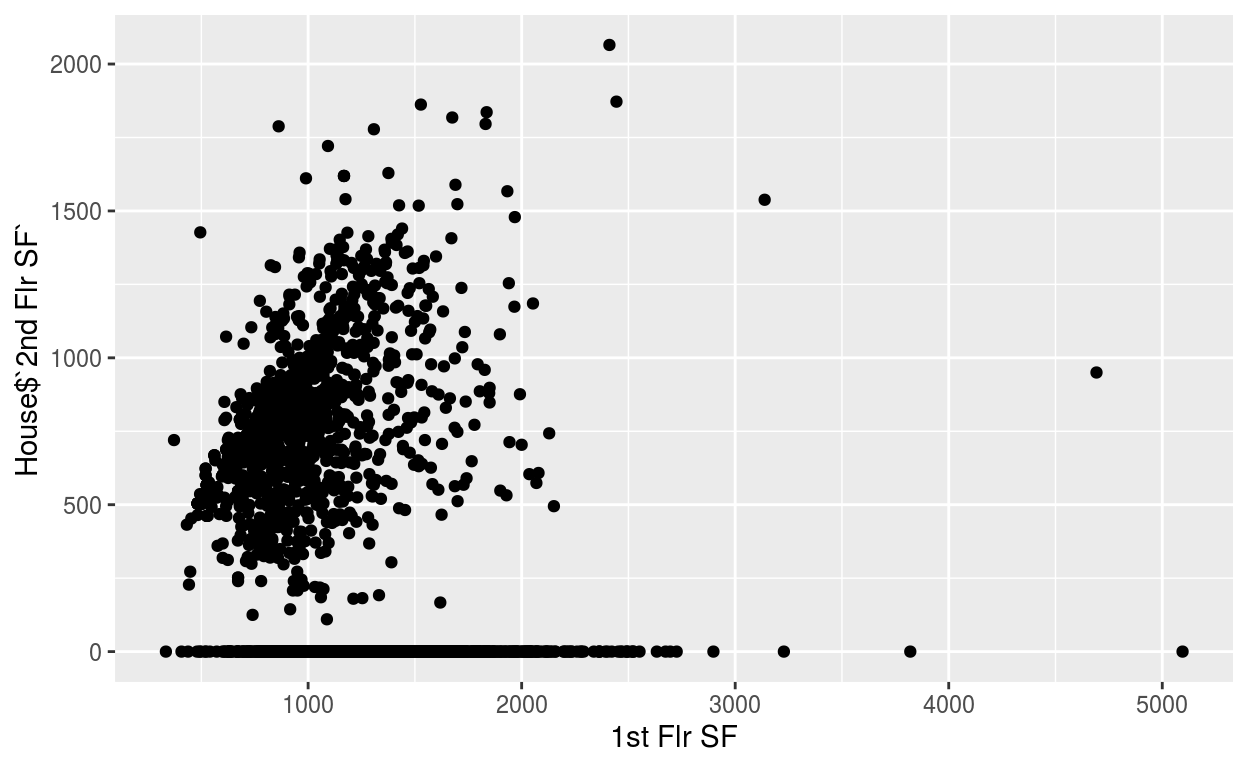
\includegraphics{HousePrice_files/figure-latex/unnamed-chunk-7-1.pdf}

분산이 일정해 보이지 않기에 SalePrice에 log를 취하겠다.

\begin{Shaded}
\begin{Highlighting}[]
\NormalTok{fit3 }\OtherTok{=} \FunctionTok{lm}\NormalTok{(}\FunctionTok{log}\NormalTok{(SalePrice) }\SpecialCharTok{\textasciitilde{}}\NormalTok{  LotArea }\SpecialCharTok{+}\NormalTok{ Street }\SpecialCharTok{+}\NormalTok{  LandContour }\SpecialCharTok{+}     
\NormalTok{              LandSlope }\SpecialCharTok{+}\NormalTok{ Neighborhood }\SpecialCharTok{+}\NormalTok{ Condition1 }\SpecialCharTok{+}\NormalTok{ Condition2 }\SpecialCharTok{+}\NormalTok{ BldgType }\SpecialCharTok{+}\NormalTok{ HouseStyle }\SpecialCharTok{+}\NormalTok{ OverallQual }\SpecialCharTok{+}  
\NormalTok{              OverallCond }\SpecialCharTok{+}\NormalTok{ YearBuilt }\SpecialCharTok{+}\NormalTok{  RoofStyle }\SpecialCharTok{+}\NormalTok{ RoofMatl }\SpecialCharTok{+}\NormalTok{ ExterQual }\SpecialCharTok{+}    
\NormalTok{              Foundation }\SpecialCharTok{+}\NormalTok{  Electrical }\SpecialCharTok{+}\NormalTok{ X1stFlrSF }\SpecialCharTok{+}\NormalTok{ X2ndFlrSF }\SpecialCharTok{+}    
\NormalTok{              LowQualFinSF }\SpecialCharTok{+}\NormalTok{  BedroomAbvGr }\SpecialCharTok{+}\NormalTok{  KitchenAbvGr }\SpecialCharTok{+} 
\NormalTok{              Fireplaces }\SpecialCharTok{+}\NormalTok{  WoodDeckSF }\SpecialCharTok{+}\NormalTok{ ScreenPorch }\SpecialCharTok{+}  
\NormalTok{              PoolArea }\SpecialCharTok{+}\NormalTok{  MoSold }\SpecialCharTok{+}\NormalTok{  SaleCondition, train)}

\FunctionTok{summary}\NormalTok{(fit3)}
\end{Highlighting}
\end{Shaded}

\begin{verbatim}
## 
## Call:
## lm(formula = log(SalePrice) ~ LotArea + Street + LandContour + 
##     LandSlope + Neighborhood + Condition1 + Condition2 + BldgType + 
##     HouseStyle + OverallQual + OverallCond + YearBuilt + RoofStyle + 
##     RoofMatl + ExterQual + Foundation + Electrical + X1stFlrSF + 
##     X2ndFlrSF + LowQualFinSF + BedroomAbvGr + KitchenAbvGr + 
##     Fireplaces + WoodDeckSF + ScreenPorch + PoolArea + MoSold + 
##     SaleCondition, data = train)
## 
## Residuals:
##      Min       1Q   Median       3Q      Max 
## -0.70790 -0.06306  0.00150  0.06864  0.70790 
## 
## Coefficients:
##                        Estimate Std. Error t value Pr(>|t|)    
## (Intercept)           1.859e+00  6.707e-01   2.772 0.005640 ** 
## LotArea               3.325e-06  5.079e-07   6.546 8.36e-11 ***
## StreetPave            1.432e-01  6.086e-02   2.353 0.018777 *  
## LandContourHLS        5.057e-02  2.675e-02   1.890 0.058928 .  
## LandContourLow        3.831e-02  3.246e-02   1.180 0.238051    
## LandContourLvl        3.328e-02  1.916e-02   1.737 0.082571 .  
## LandSlopeMod          2.981e-02  2.024e-02   1.473 0.141108    
## LandSlopeSev         -1.706e-01  5.470e-02  -3.120 0.001849 ** 
## NeighborhoodBlueste  -5.553e-03  9.710e-02  -0.057 0.954402    
## NeighborhoodBrDale   -5.814e-02  5.137e-02  -1.132 0.257897    
## NeighborhoodBrkSide  -6.510e-03  4.294e-02  -0.152 0.879516    
## NeighborhoodClearCr   5.637e-02  4.610e-02   1.223 0.221623    
## NeighborhoodCollgCr   2.339e-02  3.607e-02   0.648 0.516835    
## NeighborhoodCrawfor   1.181e-01  4.192e-02   2.817 0.004916 ** 
## NeighborhoodEdwards  -5.554e-02  3.897e-02  -1.425 0.154279    
## NeighborhoodGilbert  -1.318e-02  3.867e-02  -0.341 0.733330    
## NeighborhoodIDOTRR   -1.127e-01  4.549e-02  -2.477 0.013389 *  
## NeighborhoodMeadowV  -1.461e-01  4.819e-02  -3.032 0.002473 ** 
## NeighborhoodMitchel  -1.478e-02  4.017e-02  -0.368 0.712975    
## NeighborhoodNAmes     1.339e-02  3.799e-02   0.352 0.724551    
## NeighborhoodNoRidge   8.599e-02  4.073e-02   2.111 0.034942 *  
## NeighborhoodNPkVill   7.139e-02  5.532e-02   1.291 0.197065    
## NeighborhoodNridgHt   1.518e-01  3.672e-02   4.135 3.77e-05 ***
## NeighborhoodNWAmes   -1.905e-02  3.963e-02  -0.481 0.630722    
## NeighborhoodOldTown  -4.761e-02  4.147e-02  -1.148 0.251155    
## NeighborhoodSawyer   -1.428e-03  4.010e-02  -0.036 0.971595    
## NeighborhoodSawyerW   1.646e-02  3.848e-02   0.428 0.668872    
## NeighborhoodSomerst   8.630e-02  3.618e-02   2.385 0.017200 *  
## NeighborhoodStoneBr   1.738e-01  4.137e-02   4.200 2.84e-05 ***
## NeighborhoodSWISU    -1.857e-03  4.814e-02  -0.039 0.969240    
## NeighborhoodTimber    6.358e-02  4.154e-02   1.530 0.126139    
## NeighborhoodVeenker   1.157e-01  5.150e-02   2.246 0.024837 *  
## Condition1Feedr       2.218e-02  2.571e-02   0.863 0.388523    
## Condition1Norm        6.373e-02  2.128e-02   2.995 0.002791 ** 
## Condition1PosA        2.224e-02  5.204e-02   0.427 0.669248    
## Condition1PosN        8.191e-02  3.865e-02   2.119 0.034245 *  
## Condition1RRAe       -3.514e-02  4.558e-02  -0.771 0.440885    
## Condition1RRAn        6.479e-02  3.527e-02   1.837 0.066438 .  
## Condition1RRNe        5.201e-03  9.443e-02   0.055 0.956083    
## Condition1RRNn        1.193e-01  6.389e-02   1.867 0.062081 .  
## Condition2Feedr      -1.503e-01  1.161e-01  -1.294 0.195892    
## Condition2Norm       -1.218e-01  9.978e-02  -1.220 0.222496    
## Condition2PosA        2.720e-02  1.698e-01   0.160 0.872807    
## Condition2PosN       -9.514e-01  1.406e-01  -6.766 1.96e-11 ***
## Condition2RRAe       -6.442e-01  2.284e-01  -2.820 0.004868 ** 
## Condition2RRAn       -2.192e-01  1.638e-01  -1.339 0.180952    
## Condition2RRNn       -1.664e-01  1.360e-01  -1.224 0.221259    
## BldgType2fmCon        3.122e-02  2.908e-02   1.074 0.283154    
## BldgTypeDuplex        2.406e-02  3.156e-02   0.762 0.445978    
## BldgTypeTwnhs        -1.399e-01  2.668e-02  -5.241 1.85e-07 ***
## BldgTypeTwnhsE       -7.579e-02  1.724e-02  -4.396 1.19e-05 ***
## HouseStyle1.5Unf     -2.790e-02  3.909e-02  -0.714 0.475562    
## HouseStyle1Story     -3.688e-03  1.892e-02  -0.195 0.845499    
## HouseStyle2.5Fin     -2.280e-02  6.095e-02  -0.374 0.708455    
## HouseStyle2.5Unf      2.033e-02  4.437e-02   0.458 0.646811    
## HouseStyle2Story     -2.656e-03  1.627e-02  -0.163 0.870337    
## HouseStyleSFoyer      5.272e-02  2.867e-02   1.839 0.066146 .  
## HouseStyleSLvl        6.864e-04  2.314e-02   0.030 0.976342    
## OverallQual           6.212e-02  5.000e-03  12.424  < 2e-16 ***
## OverallCond           5.286e-02  3.716e-03  14.225  < 2e-16 ***
## YearBuilt             3.325e-03  3.136e-04  10.604  < 2e-16 ***
## RoofStyleGable       -8.109e-02  9.488e-02  -0.855 0.392923    
## RoofStyleGambrel     -1.149e-01  1.031e-01  -1.115 0.265026    
## RoofStyleHip         -7.863e-02  9.524e-02  -0.826 0.409191    
## RoofStyleMansard     -1.584e-02  1.096e-01  -0.145 0.885123    
## RoofStyleShed         4.139e-01  1.803e-01   2.295 0.021869 *  
## RoofMatlCompShg       2.339e+00  1.494e-01  15.655  < 2e-16 ***
## RoofMatlMembran       2.549e+00  2.244e-01  11.355  < 2e-16 ***
## RoofMatlMetal         2.587e+00  2.276e-01  11.367  < 2e-16 ***
## RoofMatlRoll          2.397e+00  1.971e-01  12.164  < 2e-16 ***
## RoofMatlTar&Grv       2.222e+00  1.751e-01  12.688  < 2e-16 ***
## RoofMatlWdShake       2.124e+00  1.645e-01  12.907  < 2e-16 ***
## RoofMatlWdShngl       2.415e+00  1.572e-01  15.360  < 2e-16 ***
## ExterQualFa          -1.020e-01  4.892e-02  -2.085 0.037212 *  
## ExterQualGd          -4.846e-02  2.246e-02  -2.158 0.031120 *  
## ExterQualTA          -5.270e-02  2.540e-02  -2.075 0.038182 *  
## FoundationCBlock      3.623e-03  1.569e-02   0.231 0.817457    
## FoundationPConc       5.303e-02  1.768e-02   2.999 0.002753 ** 
## FoundationSlab       -1.329e-01  3.194e-02  -4.161 3.36e-05 ***
## FoundationStone       5.538e-02  5.672e-02   0.976 0.329050    
## FoundationWood       -8.837e-02  7.701e-02  -1.147 0.251400    
## ElectricalFuseF      -9.825e-03  2.885e-02  -0.341 0.733467    
## ElectricalFuseP      -1.431e-01  8.274e-02  -1.730 0.083939 .  
## ElectricalMix        -9.674e-02  1.310e-01  -0.739 0.460253    
## ElectricalSBrkr       5.444e-03  1.498e-02   0.363 0.716422    
## X1stFlrSF             4.084e-04  1.673e-05  24.420  < 2e-16 ***
## X2ndFlrSF             2.746e-04  2.349e-05  11.691  < 2e-16 ***
## LowQualFinSF          1.819e-04  9.278e-05   1.961 0.050115 .  
## BedroomAbvGr         -1.155e-02  6.114e-03  -1.889 0.059039 .  
## KitchenAbvGr         -8.697e-02  2.787e-02  -3.121 0.001842 ** 
## Fireplaces            3.182e-02  6.920e-03   4.598 4.67e-06 ***
## WoodDeckSF            1.124e-04  3.009e-05   3.736 0.000195 ***
## ScreenPorch           3.161e-04  6.324e-05   4.999 6.52e-07 ***
## PoolArea              1.728e-04  9.314e-05   1.855 0.063807 .  
## MoSold               -1.618e-03  1.275e-03  -1.269 0.204670    
## SaleConditionAdjLand  7.089e-02  7.394e-02   0.959 0.337853    
## SaleConditionAlloca   4.414e-02  4.302e-02   1.026 0.305045    
## SaleConditionFamily   3.210e-02  3.187e-02   1.007 0.314028    
## SaleConditionNormal   7.972e-02  1.375e-02   5.796 8.44e-09 ***
## SaleConditionPartial  1.270e-01  1.953e-02   6.504 1.10e-10 ***
## ---
## Signif. codes:  0 '***' 0.001 '**' 0.01 '*' 0.05 '.' 0.1 ' ' 1
## 
## Residual standard error: 0.1268 on 1359 degrees of freedom
##   (1 observation deleted due to missingness)
## Multiple R-squared:  0.9062, Adjusted R-squared:  0.8994 
## F-statistic: 132.6 on 99 and 1359 DF,  p-value: < 2.2e-16
\end{verbatim}

\#Residual 확인

\begin{Shaded}
\begin{Highlighting}[]
\FunctionTok{plot}\NormalTok{(fit3}\SpecialCharTok{$}\NormalTok{fitted.values,fit3}\SpecialCharTok{$}\NormalTok{residuals)}
\end{Highlighting}
\end{Shaded}

\includegraphics{HousePrice_files/figure-latex/unnamed-chunk-9-1.pdf}
분산들이 비교적 안정화되었다.

\hypertarget{fit3-uxbaa8uxb378uxb85c-test-uxb370uxc774uxd130-uxc608uxce21}{%
\section{Fit3 모델로 test 데이터
예측}\label{fit3-uxbaa8uxb378uxb85c-test-uxb370uxc774uxd130-uxc608uxce21}}

\begin{Shaded}
\begin{Highlighting}[]
\FunctionTok{exp}\NormalTok{(}\FunctionTok{predict}\NormalTok{(fit3,test))}
\end{Highlighting}
\end{Shaded}

\begin{verbatim}
##          1          2          3          4          5          6          7 
##  123861.09  160762.44  174099.46  194373.67  218677.69  176438.41  181689.91 
##          8          9         10         11         12         13         14 
##  166720.81  187639.26  113951.18  180953.37  100811.44   93831.50  147208.65 
##         15         16         17         18         19         20         21 
##  126523.13  400417.40  269570.86  308210.01  297275.99  519743.68  330775.74 
##         22         23         24         25         26         27         28 
##  228991.91  179099.12  161672.33  181430.49  200814.40  346126.53  254621.17 
##         29         30         31         32         33         34         35 
##  208738.84  226010.40  198116.34  102356.66  165210.69  280935.89  279482.69 
##         36         37         38         39         40         41         42 
##  209970.08  192894.30  162773.11  152825.88  144826.29  167518.37  154589.80 
##         43         44         45         46         47         48         49 
##  259618.27  247322.19  227544.41  183984.51  236793.89  193744.80  156243.63 
##         50         51         52         53         54         55         56 
##  133681.99  139278.67  168593.94  154862.41  145089.31  234288.80  150559.51 
##         57         58         59         60         61         62         63 
##  182826.42  134860.17  204818.73  125093.98  129501.27  178824.00  117962.03 
##         64         65         66         67         68         69         70 
##  134019.26  122017.67  114783.86  108314.42  144860.00  133335.44  208873.07 
##         71         72         73         74         75         76         77 
##  115152.73  107774.16  139478.27  135198.31  138790.59  104156.42   62656.47 
##         78         79         80         81         82         83         84 
##  146887.99  201666.32  103274.94  131990.94  130688.17  178141.22   93749.55 
##         85         86         87         88         89         90         91 
##  116761.15  133204.88  138066.97  146836.74  118115.58  120506.99  104608.90 
##         92         93         94         95         96         97         98 
##  120112.70  157363.23  124919.76  169514.43  100045.31  108070.71  106992.14 
##         99        100        101        102        103        104        105 
##   82706.39  121012.93  112186.79  126252.35  117501.62  165824.26  141905.42 
##        106        107        108        109        110        111        112 
##  250601.98   82277.89  220274.32  107637.71  135505.81  120290.85  132805.77 
##        113        114        115        116        117        118        119 
##  226505.72  114518.72  218508.70  225657.25  186576.67  144356.03  151289.97 
##        120        121        122        123        124        125        126 
##  198845.67  159064.52  123980.80  277873.68  233782.34  138496.18   84616.88 
##        127        128        129        130        131        132        133 
##  106523.41  134430.38   98232.10  139134.04  102696.13  114091.15  126616.95 
##        134        135        136        137        138        139        140 
##  139478.29  112086.92  219759.94  176983.29  226382.03  170083.00  169754.80 
##        141        142        143        144        145        146        147 
##   68682.02  106497.93   68829.01  251914.46  223388.49  175511.50  184862.26 
##        148        149        150        151        152        153        154 
##  211956.99  204605.41  169264.55  134671.55  168140.39  171183.89  105517.18 
##        155        156        157        158        159        160        161 
##   91688.84   81283.76   90948.19  125076.84  139543.46  162747.42  139152.18 
##        162        163        164        165        166        167        168 
##  139655.98  256155.97  196112.56  120553.68  163156.63  182025.11  250567.89 
##        169        170        171        172        173        174        175 
##  189859.87  375123.11  248201.86  250412.18  180099.98  177371.78  164703.79 
##        176        177        178        179        180        181        182 
##  158107.54  192222.65  204592.18  200789.83  275336.95  188888.24  229969.36 
##        183        184        185        186        187        188        189 
##  258542.23  243354.07  218726.12  147060.08  153464.28  133266.62  138731.89 
##        190        191        192        193        194        195        196 
##  107127.29  123787.04   97602.04  102558.83  150317.11  135042.97  138108.11 
##        197        198        199        200        201        202        203 
##  151838.75  151087.49  136676.87  154431.33  468473.03  395109.42  367575.81 
##        204        205        206        207        208        209        210 
##  608070.17  329292.74  306079.43  338476.29  324693.43  287212.84  339795.38 
##        211        212        213        214        215        216        217 
##  272736.73  404719.86  311464.42  273206.89  200754.15  186423.74  218551.17 
##        218        219        220        221        222        223        224 
##  466099.97  351246.23  337754.78  268917.01  287649.43  211783.98  183903.46 
##        225        226        227        228        229        230        231 
##  171973.68  169576.25  178534.92  193281.58  196744.56  182806.73  174834.02 
##        232        233        234        235        236        237        238 
##  225466.31  172197.29  170532.73  176718.70  264840.78  185470.35  341478.60 
##        239        240        241        242        243        244        245 
##  306521.44  245231.93  275141.77  260861.05  264991.37  262283.60  239526.92 
##        246        247        248        249        250        251        252 
##  186692.08  221189.62  215636.35  267768.87  235170.50  245424.17  286929.16 
##        253        254        255        256        257        258        259 
##  246700.03  223673.88  205201.32  191994.39  177692.31  162436.63  207889.44 
##        260        261        262        263        264        265        266 
##  198343.20  162563.38  138358.72  138060.54  212127.76  222077.78  194616.82 
##        267        268        269        270        271        272        273 
##  158132.69  163081.19  164599.84  164679.55  116000.30  111683.47  113747.78 
##        274        275        276        277        278        279        280 
##  116433.00  119791.44  113028.88  351713.24  266850.03  282061.19  226704.13 
##        281        282        283        284        285        286        287 
##  180186.99  166717.30  171522.34  325218.19  229166.21  255771.08  226802.89 
##        288        289        290        291        292        293        294 
##  243573.81  138640.46  121071.85  276241.93  127536.16  156903.59  187168.52 
##        295        296        297        298        299        300        301 
##  161944.71  122524.09  123299.16  132125.95  173316.56  156668.63  137276.05 
##        302        303        304        305        306        307        308 
##  173016.80  175329.72  116825.04  167530.64  183127.01  231811.80  142115.74 
##        309        310        311        312        313        314        315 
##  173446.74  149992.46  116004.39  139219.18  120531.63  153940.80  141502.43 
##        316        317        318        319        320        321        322 
##  132305.99  109737.40  139247.46  113240.74  154970.13  132593.73   88885.83 
##        323        324        325        326        327        328        329 
##  122841.57  102404.50  116680.16  128802.95  153209.21   68437.41  103110.51 
##        330        331        332        333        334        335        336 
##   70433.83  174345.27  177359.17  123269.34  152945.71  137833.37  147984.03 
##        337        338        339        340        341        342        343 
##  113006.48  126197.77  114828.65  126965.68  121521.47  131588.62  157349.18 
##        344        345        346        347        348        349        350 
##  147991.80  141228.50  145134.83  120168.09  119966.88  123144.09  133872.59 
##        351        352        353        354        355        356        357 
##   97695.44  104913.94  126051.39   90700.55   69769.76  113607.45   94838.24 
##        358        359        360        361        362        363        364 
##  133650.59  119575.35   75460.08  107516.70  129505.02   62062.38  142799.58 
##        365        366        367        368        369        370        371 
##  147091.71  103412.51  100594.13  139279.14  106925.69  139314.53  171417.14 
##        372        373        374        375        376        377        378 
##   88535.05  128190.57  116863.79  120999.57  126606.23   95436.13  107104.80 
##        379        380        381        382        383        384        385 
##  112808.35  132742.67  132164.82   94100.94  124230.99  145336.50  150901.16 
##        386        387        388        389        390        391        392 
##  146273.49  199822.59   60716.38  126520.77  114158.22  146646.25  125467.65 
##        393        394        395        396        397        398        399 
##  113815.91  169796.20  169697.53  220409.44  147136.90  132054.71  118083.14 
##        400        401        402        403        404        405        406 
##  138569.30  117022.54  271420.25  257005.00  257036.61  300246.81  281602.63 
##        407        408        409        410        411        412        413 
##  227655.11  274879.12  198764.50  205639.47  229928.61  175706.18  226710.51 
##        414        415        416        417        418        419        420 
##  166426.41  201303.96  195474.56  201778.08  208748.62  125455.22  136333.73 
##        421        422        423        424        425        426        427 
##  218347.80  258337.76  194494.25  214351.10  221788.72  262325.72  205570.53 
##        428        429        430        431        432        433        434 
##  252340.98  174295.46  116711.77  125335.99  102097.64  124579.68  132395.74 
##        435        436        437        438        439        440        441 
##  144923.68  124637.04  110977.87  118973.37  159408.97  161785.65  171813.23 
##        442        443        444        445        446        447        448 
##  159935.78  229925.75  134404.31  201880.43  164469.84  220170.62  120661.97 
##        449        450        451        452        453        454        455 
##  133846.65  125891.99  238158.29  362875.43  113454.27   67461.44  285051.30 
##        456        457        458        459        460        461        462 
##   57385.98  238406.64  152557.92  190526.33  161153.37  323615.87  281128.10 
##        463        464        465        466        467        468        469 
##  277594.08  213270.73  215824.74  344133.19  135857.93  151917.92  139429.00 
##        470        471        472        473        474        475        476 
##  147492.90  150260.80  141207.25  162165.78  176287.66  164967.98  173472.41 
##        477        478        479        480        481        482        483 
##  182156.72  161691.15  275683.70  216261.98  171544.37  172240.83  224819.51 
##        484        485        486        487        488        489        490 
##  336834.45  363219.74  131411.63  136890.68  161902.74  220580.06  177513.44 
##        491        492        493        494        495        496        497 
##  240006.98  213031.04  153124.34  211347.81  130846.11  274874.39  162155.61 
##        498        499        500        501        502        503        504 
##  259939.51  141141.26  119151.30  115975.76   98971.61  108006.53   99682.20 
##        505        506        507        508        509        510        511 
##  147644.52  138725.85  281223.45  395873.42  361186.10  378590.24  477113.74 
##        512        513        514        515        516        517        518 
##  345798.05  293751.19  309961.28  562961.20  271275.33  352571.46  380227.22 
##        519        520        521        522        523        524        525 
##  326469.28  214322.78  324896.36  222520.11  223964.73  184411.54  195776.12 
##        526        527        528        529        530        531        532 
##  198353.42  197056.67  173519.10  197119.71  211043.37  236859.45  209391.15 
##        533        534        535        536        537        538        539 
##  178174.14  238348.82  189435.38  275330.32  305700.87  295825.22  254522.08 
##        540        541        542        543        544        545        546 
##  332352.26  206413.56  235460.58  263599.47  266568.22  225825.77  235159.77 
##        547        548        549        550        551        552        553 
##  260868.24  209591.33  185512.09  197916.84  151934.22  178074.25  171581.09 
##        554        555        556        557        558        559        560 
##  178063.55  191073.24  178636.22  193215.47  116734.52  129684.84  107091.23 
##        561        562        563        564        565        566        567 
##  102999.41  194372.53  135378.75  303972.22  374229.39  181100.78  153212.56 
##        568        569        570        571        572        573        574 
##  162490.97  155632.42  250109.84  222488.90  225966.51  237591.54  158575.02 
##        575        576        577        578        579        580        581 
##  220041.39  185091.19  186161.67  336419.78  207251.56  333916.47  311771.72 
##        582        583        584        585        586        587        588 
##  227549.86  168958.74  175579.11  197427.27  147120.50  133138.46  133373.00 
##        589        590        591        592        593        594        595 
##  146682.93  167859.88  110447.12  121471.70  143180.55  102906.26  146594.73 
##        596        597        598        599        600        601        602 
##  158381.75  111274.93  197799.39  131225.25  175442.70  176821.90  122758.08 
##        603        604        605        606        607        608        609 
##  117607.59  130007.71  102830.83  185697.44  145335.96  152582.22   89699.65 
##        610        611        612        613        614        615        616 
##  124371.48   97794.41  118797.80  132577.88  155964.05  139524.95  117020.76 
##        617        618        619        620        621        622        623 
##  143943.97  119024.51  128500.73  127242.76  128506.77  128050.07  144972.43 
##        624        625        626        627        628        629        630 
##  119805.35  127223.03  128235.13  120899.78  102157.46   85891.43  124240.74 
##        631        632        633        634        635        636        637 
##  106586.63  128177.69  109535.16  122647.03  132149.15  100769.26  105150.33 
##        638        639        640        641        642        643        644 
##  130663.25   65302.94   87747.15  101006.13  131070.41   99617.91  119946.24 
##        645        646        647        648        649        650        651 
##  134092.86   61999.55  174882.61  117815.02  115088.86  126911.95  176172.70 
##        652        653        654        655        656        657        658 
##  136404.29  119265.76  121026.00  158355.10  117190.21  145457.78  118612.56 
##        659        660        661        662        663        664        665 
##  118143.56  110939.08  103032.60  113631.04  108990.51  170153.32  114345.54 
##        666        667        668        669        670        671        672 
##  124712.90  172433.30  129714.66   79747.46  116942.26  134106.18  103338.14 
##        673        674        675        676        677        678        679 
##  112030.33  110995.03   87055.35   72025.57  106663.12  124377.47  145205.34 
##        680        681        682        683        684        685        686 
##  135572.21  176476.46  123897.63  152387.21  105016.50  132982.91  160629.68 
##        687        688        689        690        691        692        693 
##  141702.97  132721.06  146523.58  219297.40  123540.28  161854.91  177779.74 
##        694        695        696        697        698        699        700 
##  127012.76  141602.62  274903.53  223321.27  233804.02  234617.55  193797.71 
##        701        702        703        704        705        706        707 
##  240813.63  344535.87  317827.18  223845.91  188477.25  164046.60  201599.64 
##        708        709        710        711        712        713        714 
##  189348.22  189589.26  209595.42  148857.67  129645.56  186279.17  242846.26 
##        715        716        717        718        719        720        721 
##  268483.93  259301.54  247153.32  221980.38  139403.63  201409.00  198644.25 
##        722        723        724        725        726        727        728 
##  224478.31  193789.49  117964.61  123758.03  141425.82  146781.01  152624.83 
##        729        730        731        732        733        734        735 
##  398254.59  106352.12   87840.98   84875.48  112265.32  110310.29  101152.50 
##        736        737        738        739        740        741        742 
##  105798.88  114244.52  167578.46  152222.04  141910.17  140690.92  213619.73 
##        743        744        745        746        747        748        749 
##  133229.25  185972.88  127791.19  159217.82  218675.08  264213.42  221149.60 
##        750        751        752        753        754        755        756 
##  118478.84  112308.34  119810.74  105713.14  130595.44  101068.54  136675.19 
##        757        758        759        760        761        762        763 
##   58164.96   95487.91   90040.12   71357.27  284130.49  251504.72  246689.19 
##        764        765        766        767        768        769        770 
##  204782.93  123850.92  180961.90  194860.86  236764.16  255024.07  169012.62 
##        771        772        773        774        775        776        777 
##  215009.24  191607.28  177648.74  232377.38  211051.72  265664.90  283325.88 
##        778        779        780        781        782        783        784 
##  171273.60  149547.91  145932.99  133915.47  108892.27  131457.97   94809.71 
##        785        786        787        788        789        790        791 
##   87705.44  139092.47  115228.07  133459.71  121268.25  127325.42  106524.88 
##        792        793        794        795        796        797        798 
##  182472.04  165918.02  185885.76  174273.48  172200.87  213009.28  164276.31 
##        799        800        801        802        803        804        805 
##  179715.93  123398.89  190197.67  218022.04  335260.17  571439.49  163581.29 
##        806        807        808        809        810        811        812 
##  277275.86  393046.51  504086.59  138522.82  182389.95  197694.49  147810.87 
##        813        814        815        816        817        818        819 
##  153988.71  161075.34  148656.59  183064.52  178092.77  157046.02  118465.04 
##        820        821        822        823        824        825        826 
##  125734.90  168648.46  166847.58  108060.10  103512.51  149630.68  125110.40 
##        827        828        829        830        831        832        833 
##  350411.35  291903.27  358159.40  453855.97  348650.21  434120.86  487876.92 
##        834        835        836        837        838        839        840 
##  408605.95  466851.19  332830.61  324243.43  349707.01  392642.41  325037.02 
##        841        842        843        844        845        846        847 
##  279115.40  246101.75  276843.47  279296.68  191479.15  183525.79  201322.03 
##        848        849        850        851        852        853        854 
##  230155.73  280905.87  230464.27  214084.06  174022.10  177206.20  185422.18 
##        855        856        857        858        859        860        861 
##  183433.01  192910.84  175037.02  176100.54  185518.96  196101.90  209220.75 
##        862        863        864        865        866        867        868 
##  197072.44  176568.46  171723.68  219598.15  180083.17  205032.93  214343.83 
##        869        870        871        872        873        874        875 
##  182537.77  190124.41  334828.93  392134.88  320433.69  266951.18  272426.97 
##        876        877        878        879        880        881        882 
##  304264.51  218684.45  251607.82  238313.66  375106.24  228539.56  235464.80 
##        883        884        885        886        887        888        889 
##  229136.53  226670.51  247754.45  225500.58  212924.14  246056.00  178136.61 
##        890        891        892        893        894        895        896 
##  265170.32  277638.39  267017.55  263448.66  167967.01  173112.09  137742.00 
##        897        898        899        900        901        902        903 
##  200399.21  189358.39  142884.68  121564.31  137411.74  299039.77  115638.64 
##        904        905        906        907        908        909        910 
##  138123.14  211721.45  194791.04  230878.60  203220.05  228792.67  157282.50 
##        911        912        913        914        915        916        917 
##  156746.41  201193.56  282561.38  311241.31  240111.40  313832.79  360982.92 
##        918        919        920        921        922        923        924 
##  141101.72  201693.96  158884.59  159921.09  222964.25  217982.75  232668.96 
##        925        926        927        928        929        930        931 
##  151950.44  127283.28  134894.82  103274.86  126311.66  138042.32  137317.35 
##        932        933        934        935        936        937        938 
##  127100.68  160605.59  133915.35  202093.02  154122.35  208691.61  135389.90 
##        939        940        941        942        943        944        945 
##   73141.87   78420.34  123045.18  139131.79  141804.30  158807.52  154103.53 
##        946        947        948        949        950        951        952 
##  135734.14  121397.92  143701.56  129864.14  185043.74  114793.38  156159.02 
##        953        954        955        956        957        958        959 
##  127405.79  154177.58  135689.51  129533.39  136680.66  134730.81  124868.04 
##        960        961        962        963        964        965        966 
##  121681.12  169648.69  101982.08  105949.25  156382.86  194693.66  103940.34 
##        967        968        969        970        971        972        973 
##  124724.14  190227.23  116993.91  132884.83  114846.53  132642.55  147431.54 
##        974        975        976        977        978        979        980 
##  123875.28  145725.98  100712.17  115030.17  125282.86   99491.44  117818.86 
##        981        982        983        984        985        986        987 
##   99476.57  103248.24  134879.58  113588.20   90151.76  124954.40  173057.53 
##        988        989        990        991        992        993        994 
##  120777.28  107556.55  141429.85  121214.24  197916.76  108675.26  122585.82 
##        995        996        997        998        999       1000       1001 
##  131657.50  161142.99  124822.17  130416.76  111995.23  132781.26  133560.78 
##       1002       1003       1004       1005       1006       1007       1008 
##  136817.41  115970.17  169886.88  132139.80  110892.50  121883.86   87801.89 
##       1009       1010       1011       1012       1013       1014       1015 
##   85614.00  185698.40  214206.02  140264.12  103382.55   63445.28  224115.77 
##       1016       1017       1018       1019       1020       1021       1022 
##  125009.72  130610.75  158479.07   97532.70  148403.46  116401.41  122757.88 
##       1023       1024       1025       1026       1027       1028       1029 
##  115555.92  119418.30  124584.15  133608.93  168020.43  169307.13  143293.18 
##       1030       1031       1032       1033       1034       1035       1036 
##  135343.41   95725.93  204657.25  143130.47  151467.22  109067.49  285830.02 
##       1037       1038       1039       1040       1041       1042       1043 
##  151554.72  110228.52   88294.09  121930.79  128943.43  140937.68   91097.94 
##       1044       1045       1046       1047       1048       1049       1050 
##  194377.20  218993.38  255451.31  302360.34  256004.98  212497.67  227571.88 
##       1051       1052       1053       1054       1055       1056       1057 
##  185853.49  205770.13  215160.63  416065.98  143828.45  168966.14  159561.33 
##       1058       1059       1060       1061       1062       1063       1064 
##  161507.72  220352.82  205053.05  195455.92  216054.04  111217.72  133512.56 
##       1065       1066       1067       1068       1069       1070       1071 
##  146580.84  129535.72  119235.33  125993.47  118392.16  133685.75  241687.87 
##       1072       1073       1074       1075       1076       1077       1078 
##  219383.47  204477.79  229391.72  295334.40  242824.50  230255.09  192166.67 
##       1079       1080       1081       1082       1083       1084       1085 
##  181952.92  192837.47  191938.49  164624.80  118082.74  115589.46  123159.51 
##       1086       1087       1088       1089       1090       1091       1092 
##  134789.53  140656.95  142445.22  144849.19 1334488.30  144139.65  121460.20 
##       1093       1094       1095       1096       1097       1098       1099 
##   96341.59  104239.84  113335.13   96507.86   94851.63  167315.72  146388.69 
##       1100       1101       1102       1103       1104       1105       1106 
##  154474.68  156640.95  157792.98  162627.74  197701.68  165023.21  153305.29 
##       1107       1108       1109       1110       1111       1112       1113 
##  140424.31  193954.23  215107.14  118630.30  199177.79  146744.85  221086.47 
##       1114       1115       1116       1117       1118       1119       1120 
##  407875.41  116689.48  112490.42  119451.09   87607.16   71414.19  104597.31 
##       1121       1122       1123       1124       1125       1126       1127 
##   95688.48  118297.00  279984.45  170660.39  171165.93  208822.46  193678.73 
##       1128       1129       1130       1131       1132       1133       1134 
##  156857.68  154438.21  200106.91  296391.51  247762.67  261031.40  193111.80 
##       1135       1136       1137       1138       1139       1140       1141 
##  214405.89  286815.01  196162.27  271851.80  399882.68  187439.75  142258.45 
##       1142       1143       1144       1145       1146       1147       1148 
##   76771.61   79981.18   90372.89   74008.00  146471.40  212854.94  222668.18 
##       1149       1150       1151       1152       1153       1154       1155 
##  171318.19  130831.23  203386.68  149536.41  135766.95  126754.13  146753.57 
##       1156       1157       1158       1159       1160       1161       1162 
##  156423.45  168954.69  144506.94  215599.53  177588.10  178060.07  187935.80 
##       1163       1164       1165       1166       1167       1168       1169 
##  244358.02  292470.99  367420.26  174565.07  185175.87  438302.53  573114.28 
##       1170       1171       1172       1173       1174       1175       1176 
##  376906.40  492816.95  437177.34  291671.57  415618.68  161442.67  177849.94 
##       1177       1178       1179       1180       1181       1182       1183 
##  165233.71  273960.38  182551.71  145578.88  104495.37  172745.47  105992.29 
##       1184       1185       1186       1187       1188       1189       1190 
##  121598.66  108389.01   96241.76  103047.94  147209.17  161518.21  146833.46 
##       1191       1192       1193       1194       1195       1196       1197 
##  137127.47  401048.08  274733.83  267378.44  390527.80  333982.21  365645.25 
##       1198       1199       1200       1201       1202       1203       1204 
##  327632.46  323425.35  342733.49  354061.67  332002.59  292377.57  278425.48 
##       1205       1206       1207       1208       1209       1210       1211 
##  299277.35  305299.24  179918.64  186053.62  183852.36  272501.18  186928.17 
##       1212       1213       1214       1215       1216       1217       1218 
##  188210.06  190490.04  194271.57  167076.23  192023.40  194646.54  254723.27 
##       1219       1220       1221       1222       1223       1224       1225 
##  258722.46  275795.13  371363.21  325581.71  536944.15  298186.50  347901.31 
##       1226       1227       1228       1229       1230       1231       1232 
##  281209.63  275928.01  237057.52  222218.37  377817.10  199056.33  163960.69 
##       1233       1234       1235       1236       1237       1238       1239 
##  206597.52  157214.81  199123.82  191382.45  189922.77  187105.23  161144.76 
##       1240       1241       1242       1243       1244       1245       1246 
##  150402.82  139839.21  100427.70  144678.32  144535.06  110965.20  109044.67 
##       1247       1248       1249       1250       1251       1252       1253 
##  117647.45  128908.15  120114.62  127561.61  394005.23  374974.89  179732.29 
##       1254       1255       1256       1257       1258       1259       1260 
##  150314.38  168079.39  155392.28  216512.29  238705.27  141932.40  176166.18 
##       1261       1262       1263       1264       1265       1266       1267 
##  119023.33  152577.12  133058.86  126035.29  126682.35  150478.31  196016.21 
##       1268       1269       1270       1271       1272       1273       1274 
##  174172.08  140250.11  146957.96  134028.90  136596.62  156978.73  165315.50 
##       1275       1276       1277       1278       1279       1280       1281 
##  125152.30  155609.08  120753.36  141693.25  151590.83  143179.53  134947.46 
##       1282       1283       1284       1285       1286       1287       1288 
##  149490.10  159429.53  149537.66  136178.40  125129.79  171176.95  136247.11 
##       1289       1290       1291       1292       1293       1294       1295 
##  134810.39  122253.36  127185.05  163492.39  141647.99  179719.83  134815.19 
##       1296       1297       1298       1299       1300       1301       1302 
##   98357.97   64320.62   88204.60  141444.23   99301.16  146014.58  138337.82 
##       1303       1304       1305       1306       1307       1308       1309 
##  203857.19  152886.04  313258.66  133385.16   78622.81  137233.24  125235.23 
##       1310       1311       1312       1313       1314       1315       1316 
##  135776.02  111399.37  124314.94  145763.21  139850.38  125220.10  126664.28 
##       1317       1318       1319       1320       1321       1322       1323 
##  134798.38  132089.24  117307.76   98114.19  103382.43   99467.34   96990.33 
##       1324       1325       1326       1327       1328       1329       1330 
##  121886.97  127533.29   71253.47  130562.00   81397.21  154940.16  107652.61 
##       1331       1332       1333       1334       1335       1336       1337 
##  109116.20   57446.94  151123.35   85438.49  122782.26   98521.01  206309.71 
##       1338       1339       1340       1341       1342       1343       1344 
##   95100.34  102174.96   73832.53   98304.25  129052.68  159305.98  136642.58 
##       1345       1346       1347       1348       1349       1350       1351 
##  103974.48   92417.73  271536.32  139468.54  139762.68  118562.31  153315.40 
##       1352       1353       1354       1355       1356       1357       1358 
##  155953.60  160355.09  156747.18  103785.91  218357.41  149593.29  134937.03 
##       1359       1360       1361       1362       1363       1364       1365 
##  177616.02  124552.03  109441.32  195172.57  347717.43  154031.03  140945.80 
##       1366       1367       1368       1369       1370       1371       1372 
##  131860.05  134293.93  204340.00  217203.23  231765.71  170822.20  242701.07 
##       1373       1374       1375       1376       1377       1378       1379 
##  244773.09  220987.67  223707.04  193179.58  151971.50  157469.72  186879.85 
##       1380       1381       1382       1383       1384       1385       1386 
##  191949.37  199282.88  213598.10  156627.99  168795.75  138366.44  206855.39 
##       1387       1388       1389       1390       1391       1392       1393 
##  192702.67  217223.01  203735.22  258984.58  223429.29  222880.89  221840.71 
##       1394       1395       1396       1397       1398       1399       1400 
##  138496.18  193921.62  208522.96  194328.00  201298.26   94796.88  137244.99 
##       1401       1402       1403       1404       1405       1406       1407 
##  115770.44  190102.95  139131.67  233683.54  149901.36  157634.51  103551.35 
##       1408       1409       1410       1411       1412       1413       1414 
##   86466.57  103748.59  114144.19   87773.19   57210.79  112801.79  127545.27 
##       1415       1416       1417       1418       1419       1420       1421 
##  115190.90  163822.35  149438.24  163807.30  127856.20  106913.58  156727.28 
##       1422       1423       1424       1425       1426       1427       1428 
##  185933.63  186434.99  200384.27  194654.93  248266.70   97345.88  124310.87 
##       1429       1430       1431       1432       1433       1434       1435 
##   72794.75   81586.16  129737.94   61600.23   98259.13   66152.21  301099.84 
##       1436       1437       1438       1439       1440       1441       1442 
##  265495.53  200110.16  156820.25  208458.85  149670.74  197691.45  163582.43 
##       1443       1444       1445       1446       1447       1448       1449 
##  311852.16  320260.57  100709.24  178084.89  116500.55  124360.38  146097.38 
##       1450       1451       1452       1453       1454       1455       1456 
##   81798.76   81845.33  158709.36   73412.76   80278.62   89352.85   79384.49 
##       1457       1458       1459 
##  143690.14  142170.16  217101.70
\end{verbatim}

\#Test 데이터에 SalePrice 만들기

\begin{Shaded}
\begin{Highlighting}[]
\NormalTok{test }\SpecialCharTok{\%\textless{}\textgreater{}\%} \FunctionTok{mutate}\NormalTok{(}\AttributeTok{SalePrice =} \FunctionTok{exp}\NormalTok{(}\FunctionTok{predict}\NormalTok{(fit3,test)))}
\FunctionTok{glimpse}\NormalTok{(test)}
\end{Highlighting}
\end{Shaded}

\begin{verbatim}
## Rows: 1,459
## Columns: 81
## $ Id            <int> 1461, 1462, 1463, 1464, 1465, 1466, 1467, 1468, 1469, 14~
## $ MSSubClass    <int> 20, 20, 60, 60, 120, 60, 20, 60, 20, 20, 120, 160, 160, ~
## $ MSZoning      <chr> "RH", "RL", "RL", "RL", "RL", "RL", "RL", "RL", "RL", "R~
## $ LotFrontage   <int> 80, 81, 74, 78, 43, 75, NA, 63, 85, 70, 26, 21, 21, 24, ~
## $ LotArea       <int> 11622, 14267, 13830, 9978, 5005, 10000, 7980, 8402, 1017~
## $ Street        <chr> "Pave", "Pave", "Pave", "Pave", "Pave", "Pave", "Pave", ~
## $ Alley         <chr> NA, NA, NA, NA, NA, NA, NA, NA, NA, NA, NA, NA, NA, NA, ~
## $ LotShape      <chr> "Reg", "IR1", "IR1", "IR1", "IR1", "IR1", "IR1", "IR1", ~
## $ LandContour   <chr> "Lvl", "Lvl", "Lvl", "Lvl", "HLS", "Lvl", "Lvl", "Lvl", ~
## $ Utilities     <chr> "AllPub", "AllPub", "AllPub", "AllPub", "AllPub", "AllPu~
## $ LotConfig     <chr> "Inside", "Corner", "Inside", "Inside", "Inside", "Corne~
## $ LandSlope     <chr> "Gtl", "Gtl", "Gtl", "Gtl", "Gtl", "Gtl", "Gtl", "Gtl", ~
## $ Neighborhood  <chr> "NAmes", "NAmes", "Gilbert", "Gilbert", "StoneBr", "Gilb~
## $ Condition1    <chr> "Feedr", "Norm", "Norm", "Norm", "Norm", "Norm", "Norm",~
## $ Condition2    <chr> "Norm", "Norm", "Norm", "Norm", "Norm", "Norm", "Norm", ~
## $ BldgType      <chr> "1Fam", "1Fam", "1Fam", "1Fam", "TwnhsE", "1Fam", "1Fam"~
## $ HouseStyle    <chr> "1Story", "1Story", "2Story", "2Story", "1Story", "2Stor~
## $ OverallQual   <int> 5, 6, 5, 6, 8, 6, 6, 6, 7, 4, 7, 6, 5, 6, 7, 9, 8, 9, 8,~
## $ OverallCond   <int> 6, 6, 5, 6, 5, 5, 7, 5, 5, 5, 5, 5, 5, 6, 6, 5, 5, 5, 5,~
## $ YearBuilt     <int> 1961, 1958, 1997, 1998, 1992, 1993, 1992, 1998, 1990, 19~
## $ YearRemodAdd  <int> 1961, 1958, 1998, 1998, 1992, 1994, 2007, 1998, 1990, 19~
## $ RoofStyle     <chr> "Gable", "Hip", "Gable", "Gable", "Gable", "Gable", "Gab~
## $ RoofMatl      <chr> "CompShg", "CompShg", "CompShg", "CompShg", "CompShg", "~
## $ Exterior1st   <chr> "VinylSd", "Wd Sdng", "VinylSd", "VinylSd", "HdBoard", "~
## $ Exterior2nd   <chr> "VinylSd", "Wd Sdng", "VinylSd", "VinylSd", "HdBoard", "~
## $ MasVnrType    <chr> "None", "BrkFace", "None", "BrkFace", "None", "None", "N~
## $ MasVnrArea    <int> 0, 108, 0, 20, 0, 0, 0, 0, 0, 0, 0, 504, 492, 0, 0, 162,~
## $ ExterQual     <chr> "TA", "TA", "TA", "TA", "Gd", "TA", "TA", "TA", "TA", "T~
## $ ExterCond     <chr> "TA", "TA", "TA", "TA", "TA", "TA", "Gd", "TA", "TA", "T~
## $ Foundation    <chr> "CBlock", "CBlock", "PConc", "PConc", "PConc", "PConc", ~
## $ BsmtQual      <chr> "TA", "TA", "Gd", "TA", "Gd", "Gd", "Gd", "Gd", "Gd", "T~
## $ BsmtCond      <chr> "TA", "TA", "TA", "TA", "TA", "TA", "TA", "TA", "TA", "T~
## $ BsmtExposure  <chr> "No", "No", "No", "No", "No", "No", "No", "No", "Gd", "N~
## $ BsmtFinType1  <chr> "Rec", "ALQ", "GLQ", "GLQ", "ALQ", "Unf", "ALQ", "Unf", ~
## $ BsmtFinSF1    <int> 468, 923, 791, 602, 263, 0, 935, 0, 637, 804, 1051, 156,~
## $ BsmtFinType2  <chr> "LwQ", "Unf", "Unf", "Unf", "Unf", "Unf", "Unf", "Unf", ~
## $ BsmtFinSF2    <int> 144, 0, 0, 0, 0, 0, 0, 0, 0, 78, 0, 0, 0, 0, 0, 0, 0, 0,~
## $ BsmtUnfSF     <int> 270, 406, 137, 324, 1017, 763, 233, 789, 663, 0, 354, 32~
## $ TotalBsmtSF   <int> 882, 1329, 928, 926, 1280, 763, 1168, 789, 1300, 882, 14~
## $ Heating       <chr> "GasA", "GasA", "GasA", "GasA", "GasA", "GasA", "GasA", ~
## $ HeatingQC     <chr> "TA", "TA", "Gd", "Ex", "Ex", "Gd", "Ex", "Gd", "Gd", "T~
## $ CentralAir    <chr> "Y", "Y", "Y", "Y", "Y", "Y", "Y", "Y", "Y", "Y", "Y", "~
## $ Electrical    <chr> "SBrkr", "SBrkr", "SBrkr", "SBrkr", "SBrkr", "SBrkr", "S~
## $ X1stFlrSF     <int> 896, 1329, 928, 926, 1280, 763, 1187, 789, 1341, 882, 13~
## $ X2ndFlrSF     <int> 0, 0, 701, 678, 0, 892, 0, 676, 0, 0, 0, 504, 567, 601, ~
## $ LowQualFinSF  <int> 0, 0, 0, 0, 0, 0, 0, 0, 0, 0, 0, 0, 0, 0, 0, 0, 0, 0, 0,~
## $ GrLivArea     <int> 896, 1329, 1629, 1604, 1280, 1655, 1187, 1465, 1341, 882~
## $ BsmtFullBath  <int> 0, 0, 0, 0, 0, 0, 1, 0, 1, 1, 1, 0, 0, 0, 0, 0, 0, 0, 0,~
## $ BsmtHalfBath  <int> 0, 0, 0, 0, 0, 0, 0, 0, 0, 0, 0, 0, 0, 0, 0, 0, 0, 0, 0,~
## $ FullBath      <int> 1, 1, 2, 2, 2, 2, 2, 2, 1, 1, 2, 1, 1, 2, 1, 2, 2, 2, 2,~
## $ HalfBath      <int> 0, 1, 1, 1, 0, 1, 0, 1, 1, 0, 0, 1, 1, 1, 0, 1, 0, 0, 0,~
## $ BedroomAbvGr  <int> 2, 3, 3, 3, 2, 3, 3, 3, 2, 2, 2, 2, 3, 3, 2, 3, 3, 3, 3,~
## $ KitchenAbvGr  <int> 1, 1, 1, 1, 1, 1, 1, 1, 1, 1, 1, 1, 1, 1, 1, 1, 1, 1, 1,~
## $ KitchenQual   <chr> "TA", "Gd", "TA", "Gd", "Gd", "TA", "TA", "TA", "Gd", "T~
## $ TotRmsAbvGrd  <int> 5, 6, 6, 7, 5, 7, 6, 7, 5, 4, 5, 5, 6, 6, 4, 10, 7, 7, 8~
## $ Functional    <chr> "Typ", "Typ", "Typ", "Typ", "Typ", "Typ", "Typ", "Typ", ~
## $ Fireplaces    <int> 0, 0, 1, 1, 0, 1, 0, 1, 1, 0, 1, 0, 0, 1, 0, 1, 0, 1, 1,~
## $ FireplaceQu   <chr> NA, NA, "TA", "Gd", NA, "TA", NA, "Gd", "Po", NA, "Fa", ~
## $ GarageType    <chr> "Attchd", "Attchd", "Attchd", "Attchd", "Attchd", "Attch~
## $ GarageYrBlt   <int> 1961, 1958, 1997, 1998, 1992, 1993, 1992, 1998, 1990, 19~
## $ GarageFinish  <chr> "Unf", "Unf", "Fin", "Fin", "RFn", "Fin", "Fin", "Fin", ~
## $ GarageCars    <int> 1, 1, 2, 2, 2, 2, 2, 2, 2, 2, 2, 1, 1, 2, 1, 3, 3, 3, 3,~
## $ GarageArea    <int> 730, 312, 482, 470, 506, 440, 420, 393, 506, 525, 511, 2~
## $ GarageQual    <chr> "TA", "TA", "TA", "TA", "TA", "TA", "TA", "TA", "TA", "T~
## $ GarageCond    <chr> "TA", "TA", "TA", "TA", "TA", "TA", "TA", "TA", "TA", "T~
## $ PavedDrive    <chr> "Y", "Y", "Y", "Y", "Y", "Y", "Y", "Y", "Y", "Y", "Y", "~
## $ WoodDeckSF    <int> 140, 393, 212, 360, 0, 157, 483, 0, 192, 240, 203, 275, ~
## $ OpenPorchSF   <int> 0, 36, 34, 36, 82, 84, 21, 75, 0, 0, 68, 0, 0, 0, 30, 13~
## $ EnclosedPorch <int> 0, 0, 0, 0, 0, 0, 0, 0, 0, 0, 0, 0, 0, 0, 0, 0, 0, 0, 0,~
## $ X3SsnPorch    <int> 0, 0, 0, 0, 0, 0, 0, 0, 0, 0, 0, 0, 0, 0, 0, 0, 0, 0, 0,~
## $ ScreenPorch   <int> 120, 0, 0, 0, 144, 0, 0, 0, 0, 0, 0, 0, 0, 0, 0, 0, 0, 0~
## $ PoolArea      <int> 0, 0, 0, 0, 0, 0, 0, 0, 0, 0, 0, 0, 0, 0, 0, 0, 0, 0, 0,~
## $ PoolQC        <chr> NA, NA, NA, NA, NA, NA, NA, NA, NA, NA, NA, NA, NA, NA, ~
## $ Fence         <chr> "MnPrv", NA, "MnPrv", NA, NA, NA, "GdPrv", NA, NA, "MnPr~
## $ MiscFeature   <chr> NA, "Gar2", NA, NA, NA, NA, "Shed", NA, NA, NA, NA, NA, ~
## $ MiscVal       <int> 0, 12500, 0, 0, 0, 0, 500, 0, 0, 0, 0, 0, 0, 0, 0, 0, 0,~
## $ MoSold        <int> 6, 6, 3, 6, 1, 4, 3, 5, 2, 4, 6, 2, 3, 6, 6, 1, 6, 6, 2,~
## $ YrSold        <int> 2010, 2010, 2010, 2010, 2010, 2010, 2010, 2010, 2010, 20~
## $ SaleType      <chr> "WD", "WD", "WD", "WD", "WD", "WD", "WD", "WD", "WD", "W~
## $ SaleCondition <chr> "Normal", "Normal", "Normal", "Normal", "Normal", "Norma~
## $ SalePrice     <dbl> 123861.1, 160762.4, 174099.5, 194373.7, 218677.7, 176438~
\end{verbatim}

SalePrice열 확인

\#Csv 파일 생성

\begin{Shaded}
\begin{Highlighting}[]
\FunctionTok{write.csv}\NormalTok{(test, }\StringTok{"prediction.csv"}\NormalTok{)}
\end{Highlighting}
\end{Shaded}

\#Submission 규격에 맞게 파일 생성

\begin{Shaded}
\begin{Highlighting}[]
\NormalTok{ForSubmission }\OtherTok{=}\NormalTok{ test }\SpecialCharTok{\%\textgreater{}\%} \FunctionTok{select}\NormalTok{(Id, SalePrice)}
\FunctionTok{write.csv}\NormalTok{(ForSubmission, }\StringTok{"ForSubmission.csv"}\NormalTok{)}
\end{Highlighting}
\end{Shaded}


<!--radix_placeholder_site_after_body-->
<!--/radix_placeholder_site_after_body-->

<!--radix_placeholder_navigation_after_body-->
<!--/radix_placeholder_navigation_after_body-->

\end{document}
